\appendix
\section*{Appendix}

\begin{itemize}
    \item[] \ref{appendix:sec:additional_background} Additional background
    \begin{itemize}
        \item[] \ref{appendix:subsec:group_theory} Group theory 
        \item[] \ref{appendix:subsec:equivariance} Equivariance
        \item[] \ref{appendix:subsec:equivariant_irreps_feature} Equivariant features based on vector spaces of irreducible representations
        \item[] \ref{appendix:subsec:tensor_product} Tensor product
    \end{itemize}
    \item[] \ref{appendix:sec:related_works} Related works
    \begin{itemize}
        \item[] \ref{appendix:subsec:gnn_3d_graphs} Graph neural networks for 3D atomistic graphs
        \item[] \ref{appendix:subsec:detailed_comparison_between_equivariant_transformers} \revision{Detailed comparison between equivariant Transformers}
        \item[] \ref{appendix:subsec:invariant_gnn} Invariant GNNs
        \item[] \ref{appendix:subsec:attention_and_transformers} Attention and Transformer
    \end{itemize}
    \item[] \ref{appendix:sec:details_architecture} Details of architecture
    \begin{itemize}
        \item[] \ref{appendix:subsec:equivariant_operations} Equivariant operation used in Equiformer
        \item[] \ref{appendix:subsec:equiformer_architecture} Equiformer architecture
        \item[] \ref{appendix:subsec:dot_product_attention} Dot product attention
        \item[] \ref{appendix:subsec:incorporating_e3_equivariance} \revision{Incorporating E(3)-Equivariance}
        \item[] \ref{appendix:subsec:computational_complexity} Discussion on computational complexity
    \end{itemize}

    \item[] \ref{appendix:sec:qm9} Details of experiments on QM9
    \begin{itemize}
        \item[] \ref{appendix:subsec:qm9_training_details} Training details
        \item[] \ref{appendix:subsec:e3_qm9} Comparison between $SE(3)$ and $E(3)$ equivariance
        \item[] \ref{appendix:subsec:qm9_training_time_comparison} Comparison of training time and numbers of parameters
    \end{itemize}
    \item[] \ref{appendix:sec:md17} Details of experiments on MD17
    \begin{itemize}
        \item[] \ref{appendix:subsec:md17_training_details} Training details
        \item[] \ref{appendix:subsec:md17_torchmdnet} Additional comparison of performance to TorchMD-NET
        \item[] \ref{appendix:subsec:md17_training_time_comparison} Comparison of training time and numbers of parameters
    \end{itemize}
    \item[] \ref{appendix:sec:oc20} Details of experiments on OC20
    \begin{itemize}
        \item[] \ref{appendix:subsec:oc20_dataset_details} Detailed description of OC20 dataset
        \item[] \ref{appendix:subsec:oc20_training_details} Training details
        \item[] \ref{appendix:subsec:is2re_validation} Results on IS2RE validation set
        \item[] \ref{appendix:subsec:e3_oc20} Comparison between $SE(3)$ and $E(3)$ equivariance
        \item[] \ref{appendix:subsec:oc20_training_time_comparison} Comparison of training time and numbers of parameters
        \item[] \ref{appendix:subsec:error_distributions} Error distributions
    \end{itemize}
    \item[]
    \ref{appendix:sec:limitations} Limitations
    
    
\end{itemize}


\begin{comment}
Our implementation is based on PyTorch~\cite{pytorch}, PyG~\cite{pytorch_geometric}, \texttt{e3nn}~\cite{e3nn} and \texttt{timm}~\cite{timm}.
We include code for experiments on QM9 in appendix and will release code reproducing all main results in the future.

Additionally, we update the results of IS2RE with IS2RS auxiliary task by using Noisy Nodes~\cite{noisy_nodes} data augmentation and summarize them in Table~\ref{appendix:tab:is2re_is2rs_val} and~\ref{appendix:tab:is2re_is2rs_test}.
As of May 20, 2022, Equiformer achieves the best results on IS2RE task when only IS2RE and IS2RS data are used.


\begin{table}[h]
\centering
\resizebox{\ifdim\width>\textwidth\textwidth\else\width\fi}{!}{
\begin{tabular}{lccccc|ccccc}
%\cline{7-11}
\toprule[1.2pt]
 & \multicolumn{5}{c|}{Energy MAE (eV) $\downarrow$} & \multicolumn{5}{c}{EwT (\%) $\uparrow$} \\ 
\cmidrule[0.6pt]{2-11}
Methods & ID & OOD Ads & OOD Cat & OOD Both & Average & ID & OOD Ads & OOD Cat & OOD Both & Average \\
\midrule[1.2pt]
GNS~\cite{noisy_nodes} & 0.54 & 0.65 & 0.55 & 0.59 & 0.5825 & - & - & - & - & -\\
%GNS + Noisy Nodes~\cite{noisy_nodes} & 0.48 & 0.53 & 0.49 & 0.48 & 0.4950 & - & - & - & - & - \\

Noisy Nodes~\cite{noisy_nodes} & 0.47 & 0.51 & 0.48 & 0.46 & 0.4800 & - & - & - & - & - \\
Graphormer~\cite{graphormer_3d} & 0.4329 & 0.5850 & 0.4441 & 0.5299 & 0.4980 & - & - & - & - & -\\
\midrule[0.6pt]
%Equiformer& 0.5093& 0.6285 & 0.5053 & 0.5556 & 0.5497 & 5.04 & 2.85 & 4.90 & 3.04 & \\
Equiformer & 0.4222 & 0.5420 & 0.4231 & 0.4754 & 0.4657 & 7.23 & 3.77 & 7.13 & 4.10 & 5.56 \\
+ Noisy Nodes & 0.4156 &  0.4976 & 0.4165 & 0.4344 & 0.4410 & 7.47 & 4.64 & 7.19 & 4.84 & 6.04 \\
%\midrule[0.6pt]
%Equiformer + NAT & 0.4685 & 0.6071 & 0.4746 & 0.5345 & 0.5212 & 5.83 & 3.18 & 5.88 & 3.43 & \\
\bottomrule[1.2pt]
\end{tabular}
}
\vspace{2mm}
\caption{\textbf{Results on OC20 IS2RE \underline{validation} set when IS2RS node-level auxiliary task is adopted during training.} 
``GNS'' denotes the 50-layer GNS trained without Noisy Nodes data augmentation, and ``Noisy Nodes'' denotes the 100-layer GNS trained with Noisy Nodes.
Compared to the main text, we add the result of ``Equiformer + Noisy Nodes'', which use data augmentation of interpolating between initial structure and relaxed struture and adding Gaussian noise as described by Noisy Nodes~\cite{noisy_nodes}.
}

\label{appendix:tab:is2re_is2rs_val}
\end{table}


\begin{table}[h]
\centering
\resizebox{\ifdim\width>\textwidth\textwidth\else\width\fi}{!}{
\begin{tabular}{lccccc|ccccc}
%\cline{7-11}
\toprule[1.2pt]
 & \multicolumn{5}{c|}{Energy MAE (eV) $\downarrow$} & \multicolumn{5}{c}{EwT (\%) $\uparrow$} \\ 
\cmidrule[0.6pt]{2-11}
Methods & ID & OOD Ads & OOD Cat & OOD Both & Average & ID & OOD Ads & OOD Cat & OOD Both & Average \\
\midrule[1.2pt]
GNS + Noisy Nodes~\cite{noisy_nodes} & 0.4219 & 0.5678 & 0.4366 & 0.4651 & 0.4728 & 9.12 & 4.25 & 8.01 & 4.64 & 6.5 \\
%GNS + Noisy Nodes~\cite{noisy_nodes} & 0.48 & 0.53 & 0.49 & 0.48 & 0.4950 & - & - & - & - & - \\
%
%Noisy Nodes~\cite{noisy_nodes} & 0.47 & 0.51 & 0.48 & 0.46 & 0.4800 & - & - & - & - & - \\
Graphormer~\cite{graphormer_3d}$^\dagger$ & 0.3976 & 0.5719 & 0.4166 & 0.5029 & 0.4722 & 8.97 & 3.45 & 8.18 & 3.79 & 6.1\\
\midrule[0.6pt]
%Equiformer& 0.5093& 0.6285 & 0.5053 & 0.5556 & 0.5497 & 5.04 & 2.85 & 4.90 & 3.04 & \\
Equiformer + Noisy Nodes & 0.4171 & 0.5479 & 0.4248 & 0.4741 & 0.4660 & 7.71& 3.70 & 7.15 & 4.07 & 5.66 \\
%+ Noisy Nodes & 0.4156 &  0.4976 & 0.4165 & 0.4344 & 0.4410 & 7.47 & 4.64 & 7.19 & 4.84 & \\
%\midrule[0.6pt]
%Equiformer + NAT & 0.4685 & 0.6071 & 0.4746 & 0.5345 & 0.5212 & 5.83 & 3.18 & 5.88 & 3.43 & \\
\bottomrule[1.2pt]
\end{tabular}
}
\vspace{2mm}
\caption{\textbf{Results on OC20 IS2RE \underline{testing} set when IS2RS node-level auxiliary task is adopted during training.} 
$\dagger$ denotes using ensemble of models trained with both IS2RE training and validation sets.
In contrast, we use the same single Equiformer model in Table~\ref{appendix:tab:is2re_is2rs_val}, which is trained with only the training set, for evaluation on the testing set.
}

\label{appendix:tab:is2re_is2rs_test}
\end{table}

\end{comment}



\section{Additional Background}
\label{appendix:sec:additional_background}

%We provide more details on background here, and we note that they are introduced in a way that facilitates discussing the proposed method and that other works~\cite{tfn, 3dsteerable, kondor2018clebsch, cormorant, se3_transformer, segnn} also provide relevant mathematical background, which helps the presentation of this work.   

%%%In this section, we provide additional mathematical background on group equivariance helpful for the discussion of the proposed method.
In this section, we provide additional mathematical background helpful for the discussion of the proposed method.
Other works~\citep{tfn, 3dsteerable, kondor2018clebsch, cormorant, se3_transformer, segnn} also provide similar background.
We encourage interested readers to see these works~\citep{zee, Dresselhaus2007} for more in-depth and pedagogical presentations.

\subsection{Group Theory}
\label{appendix:subsec:group_theory}

\paragraph{Definition of Groups.}
A group is an algebraic structure that consists of a set $G$ and a binary operator $\circ: G \times G \rightarrow G$ and is typically denoted as $G$.
Groups satisfy the following four axioms:
\begin{enumerate}
    \item Closure: $g \circ h \in G$ for all $g, h \in G$.
    \item Identity: There exists an identity element $e \in G$ such that $g \circ e = e \circ g = g$ for all $g \in G$.
    \item Inverse: For each $g \in G$, there exists an inverse element $g^{-1} \in G$ such that $g \circ g^{-1} = g^{-1} \circ g = e$.
    \item Associativity: $f \circ g \circ h = (f \circ g) \circ h = f \circ (g \circ h )$ for all $f, g, h \in G$.
\end{enumerate}

In this work, we focus on 3D rotation, translation and inversion.
Relevant groups include:
\begin{enumerate}
    \item The Euclidean group in three dimensions $E(3)$: 3D rotation, translation and inversion.
    \item The special Euclidean group in three dimensions $SE(3)$: 3D rotation and translation.
    \item The orthogonal group in three dimensions  $O(3)$: 3D rotation and inversion.
    \item The special orthogonal group in three dimensions  $SO(3)$: 3D rotation.
    %\item The translational group $T(3)$: 3D translation.
\end{enumerate}


\paragraph{Group Representations.}
%Groups can be used to define transformations.
The actions of groups define transformations.
Formally, a transformation acting on vector space $X$ parametrized by group element $g \in G$ is an injective function $T_{g}: X \rightarrow X$.
A powerful result of group representation theory is that these transformations can be expressed as matrices which act on vector spaces via matrix multiplication. 
These matrices are called the group representations.
Formally, a group representation $D: G \rightarrow GL(N)$ is a mapping between a group $G$ and a set of $N \times N$ invertible matrices.
The group representation $D(g): X \rightarrow X$ maps an $N$-dimensional vector space $X$ onto itself and satisfies  $D(g)D(h) = D(g \circ h)$ for all $g, h \in G$.

%There are many ways to represent a group. 
%If there exists a change of basis $P$ in the form of an $N \times N$ matrix for a given representation $D(g)$ such that $P^{-1} D(g) P = D'(g)$
How a group is represented depends on the vector space it acts on.
If there exists a change of basis $P$ in the form of an $N \times N$ matrix such that $P^{-1} D(g) P = D'(g)$ for all $g \in G$, then we say the two group representations are equivalent.
If $D'(g)$ is block diagonal, which means that $g$ acts on independent subspaces of the vector space, the representation $D(g)$ is reducible.
%that makes $D'(g)$ block diagonal for all $g \in G$, meaning $g$ acts on independent subspaces of the vector space, the representation $D(g)$ is deemed reducible. 
%A particular class of representations that are convenient for generalizable and composable functions are irreducible representations or ``irreps'', which cannot be further reduced. 
A particular class of representations that are convenient for composable functions are irreducible representations or ``irreps'', which cannot be further reduced. 
We can express any group representation of $SO(3)$ as a direct sum (concatentation) of irreps \citep{zee,Dresselhaus2007,e3nn}:
\begin{equation}
D(g) = P ^{-1} \left ( \bigoplus_{i} D_{l_i}(g) \right)  P = 
P^{-1}
\begin{pmatrix}
D_{l_0}(g) & & \\
& D_{l_1}(g) & & \\
& & ...... \\
\end{pmatrix}
P
\end{equation}
where $D_{l_i}(g)$ are Wigner-D matrices with degree $l_i$ as metnioned in Sec.~\ref{subsec:irreducible_representations}.

% already mention in background
%\paragraph{Irreducible Representations of $SO(3)$.}



\subsection{Equivariance}
\label{appendix:subsec:equivariance}


\paragraph{Definition of Equivariance and Invariance.}
Equivariance is a property of a function $f: X \rightarrow Y$ mapping between vector spaces $X$ and $Y$.
Given a group $G$ and group representations $D_{X}(g)$ and $D_{Y}(g)$ in input and output spaces $X$ and $Y$, $f$ is equivariant to G if $D_Y(g) f(x) = f(D_X(g)x)$ for all $x \in X$ and $g \in G$.
%Invariance corresponds to the case that $f(x) = D_Y(g) f(x) = f(D_X(g) x)$.
Invariance corresponds to the case where $D_Y(g)$ is the identity $I$ for all $g \in G$.


\paragraph{Equivariance in Neural Networks.}
%Including equivariance in neural networks can enable generalizaing to unseen data in a predictable manner.
%For instance, an equivariant neural network $f: X \rightarrow Y$ predicts output $y$ given input $x$.
%When the input becomes $D_X(g) x$, which might not exist in training sets, $f$ can generalize to the input and predict $D_Y(g) f(x)$.
Group equivariant neural networks are guaranteed to to make equivariant predictions on data transformed by a group.
Additionally, they are found to be data-efficient and generalize better than non-symmetry-aware and invariant methods~\citep{nequip, quantum_scaling, neural_scale_of_chemical_models}.
For 3D atomistic graphs, we consider equivariance to the Euclidean group $E(3)$, which consists of 3D rotation, translation and inversion.
For translation, we operate on relative positions and therefore our networks are invariant to 3D translation.
%As for rotation and inversion, we incorporate vector spaces of $O(3)$ irreps into networks so that intermediate features and outputs are equivariant to 3D rotation and inversion.
We achieve equivariance to rotation and inversion by representing our input data, intermediate features and outputs in vector spaces of $O(3)$ irreps and acting on them with only equivariant operations. 


\subsection{Equivariant Features Based on Vector Spaces of Irreducible Representations}
\label{appendix:subsec:equivariant_irreps_feature}


\paragraph{Irreducible Representations of Inversion.}
The group of inversion $\mathbb{Z}_2$ only has two elements, identity and inversion, and two irreps, even $e$ and odd $o$.
Vectors transformed by irrep $e$ do not change sign under inversion while those by irrep $o$ do.
We create irreps of $O(3)$ by simply multiplying those of $SO(3)$ and $\mathbb{Z}_2$ and introduce parity $p$ to type-$L$ vectors to denote how they transform under inversion.
%Therefore for $O(3)$, type-$L$ vectors in $SO(3)$ are extended to type-$(L, p)$ vectors, where $p$ is $e$ or $o$.
Thus, type-$L$ vectors in $SO(3)$ become type-$(L, p)$ vectors in $O(3)$, where $p$ is $e$ or $o$.
%In the following, we use type-$L$ vectors for the ease of discussion, but we can generalize to type-$(L, p)$ vectors, unless otherwise stated.}

\paragraph{Irreps Features.}
As discussed in Sec.~\ref{subsec:irreducible_representations} in the main text, we use type-$L$ vectors for $SE(3)$-equivariant irreps features\footnote{In SEGNN~\citep{segnn}, they are also referred to as steerable features. We use the term ``irreps features'' to remain consistent with \texttt{e3nn}~\citep{e3nn} library.} and type-$(L, p)$ vectors for $E(3)$-equivariant irreps features.
Parity $p$ denotes whether vectors change sign under inversion and can be either $e$ (even) or $o$ (odd).
Vectors with $p = o$ change sign under inversion while those with $p = e$ do not.
Scalar features correspond to type-$0$ vectors in the case of $SE(3)$-equivariance and correspond to type-$(0, e)$ in the case of $E(3)$-equivariance whereas type-$(0, o)$ vectors correspond to pseudo-scalars.
Euclidean vectors in $\mathbb{R}^3$ correspond to type-$1$ vectors and type-$(1, o)$ vectors whereas type-$(1, e)$ vectors correspond to pseudo-vectors.
Note that type-$(L, e)$ vectors and type-$(L, o)$ vectors are considered vectors of different types in equivariant linear layers and layer normalizations.

\paragraph{Spherical Harmonics.}
Euclidean vectors $\vec{r}$ in $\mathbb{R}^3$ can be projected into type-$L$ vectors $f^{(L)}$ by using spherical harmonics $Y^{(L)}$: $f^{(L)} = Y^{(L)}(\frac{\vec{r}}{|| \vec{r} ||})$~\citep{finding_symmetry_breaking_order}.
This is equivalent to the Fourier transform of the angular degree of freedom $\frac{\vec{r}}{|| \vec{r}||}$, which can be optionally weighted by $|| \vec{r} ||$. 
In the case of $SE(3)$-equivariance, $f^{(L)}$ transforms in the same manner as type-$L$ vectors.
For $E(3)$-equivariance, $f^{(L)}$ behaves as type-$(L, p)$ vectors, where $p = e$ if $L$ is even and $p = o$ if $L$ is odd.
\revision{
Visualization of spherical harmonics can be found in this \href{https://docs.e3nn.org/en/latest/api/o3/o3_sh.html}{website}.}

%\paragraph{\todo{Spherical Harmonics are Wigner-D matrices.}}

\paragraph{Vectors of Higher $L$ and Other Parities.}
%So far we have restricted concrete examples of $O(3)$ irreps to commonly encountered scalars ($L=0$, $p=1$) and vectors ($L=1$, $p=-1$); irreps of higher $L$'s and other parities are equally physical. 
Although previously we have restricted concrete examples of vector spaces of $O(3)$ irreps to commonly encountered scalars (type-$(0, e)$ vectors) and Euclidean vectors (type-$(1, o)$ vectors), vector of higher $L$ and other parities are equally physical. 
%Many physical properties are described using Cartesian tensors
For example, the moment of inertia (how an object rotates under torque) transforms as a $3\times3$ symmetric matrix, which has symmetric-traceless components behaving as type-$(2, e)$ vectors.
Elasticity (how an object deforms under loading) transforms as a rank-4 or $3\times3\times3\times3$ symmetric tensor, which includes components acting as type-$(4, e)$ vectors.
%As an example, many physical properties are described using Cartesian tensors, e.g. the moment of inertia (how an object rotates under torque) transforms as a $3\times3$ symmetric matrix and elasticity (how an object deforms under loading) transforms as a rank-4 or $3\times3\times3\times3$ symmetric tensor, which have components that transform as ($L=2$, $p=1$) and ($L=4$, $p=1$), respectively. 
%\todo{More generally speaking, if one considers polynomials of distinguishable 3D vectors $\vec{x}^{(i)}$, specific linear combinations of monomials will transform as specific irreps of $O(3)$. In fact, the spherical harmonics are a specific subset of these polynomials where the inputs are identical $\vec{x}^(i) \rightarrow \vec{x}$ and the degree of the polynomial matches the $L$ of the irrep (e.g. $xy$ is of degree 2 and transforms as a component of ($L=2$, $p=1$)) \cite{e3nn}.}


\subsection{Tensor Product}
\label{appendix:subsec:tensor_product}

\paragraph{Tensor Product for $O(3)$.}
We use tensor products to interact different type-$(L, p)$ vectors.
We extend our discussion in Sec.~\ref{subsec:tensor_product} in the main text to include inversion and type-$(L, p)$ vectors.
The tensor product denoted as $\otimes$ uses Clebsch-Gordan coefficients to combine type-$(L_1, p_1)$ vector $f^{(L_1, p_1)}$ and type-$(L_2, p_2)$ vector $g^{(L_2, p_2)}$ and produces type-$(L_3, p_3)$ vector $h^{(L_3, p_3)}$ as follows:
\begin{equation}
%\begin{aligned}
h^{(L_3, p_3)}_{m_3} = (f^{(L_1, p_1)} \otimes g^{(L_2, p_2)})_{m_3} = \sum_{m_1 = -L_1}^{L_1} \sum_{m_2 = -L_2}^{L_2} C^{(L_3, m_3)}_{(L_1, m_1)(L_2, m_2)} f^{(L_1, p_1)}_{m_1} g^{(L_2, p_2)}_{m_2} 
\label{appendix:eq:tensor_product}
\end{equation}

\begin{equation}
p_3 = p_1 \times p_2
\label{appendix:eq:parity}
\end{equation}

The only difference of tensor products for $O(3)$ as described in Eq.~\ref{appendix:eq:tensor_product} from those for $SO(3)$ described in Eq.~\ref{eq:tensor_product} is that we additionally keep track of the output parity $p_3$ as in Eq.~\ref{appendix:eq:parity} and use the following multiplication rules: $e \times e = e$, $o \times o = e$, and $e \times o = o \times e = o$.
For example, the tensor product of a type-$(1, o)$ vector and a type-$(1, e)$ vector can result in one type-$(0, o)$ vector, one type-$(1, o)$ vector, and one type-$(2, o)$ vector.


\paragraph{Clebsch-Gordan Coefficients.}
The Clebsch-Gordan coefficients for $SO(3)$ are computed from integrals over the basis functions of a given irreducible representation, e.g., the real spherical harmonics, as shown below and are tabulated to avoid unnecessary computation.
\begin{equation}
     C_{(L_1, m_1) (L_2, m_2)}^{(L_3, m_3)} = \left|L_1 m_1; L_2 m_2 \right> \left<L_3 m_3 \right| = \int d{\Omega} Y^{(L_1)*}_{m_1}(\Omega) Y^{(L_2)*}_{m_2}(\Omega) Y^{(L_3)}_{m_3}(\Omega)
\end{equation}
For many combinations of $L_1$, $L_2$, and $L_3$, the Clebsch-Gordan coefficients are zero. The gives rise to the following selection rule for non-trivial coefficients: $-|L_1 + L_2| \leq L_3 \leq |L_1 + L_2|$.


\paragraph{Examples of Tensor Products.}
Tensor products generally define the interaction between different type-$(L, p)$ vectors in a symmetry-preserving manner and consist of common operations as follows:
\begin{enumerate}
    \item Scalar-scalar multiplication: scalar $(L=0, p = e)$ $\otimes$ scalar $(L=0, p=e)$ $\rightarrow$ scalar $(L=0, p=e)$.
    \item Scalar-vector multiplication: scalar $(L=0, p = e)$ $\otimes$ vector $(L=1, p=o)$ $\rightarrow$ vector $(L=1, p=o)$.
    \item Vector dot product: vector $(L=1, p = o)$ $\otimes$ vector $(L=1, p=o)$ $\rightarrow$ scalar $(L=0, p=e)$.
    \item Vector cross product: vector $(L=1, p = o)$ $\otimes$ vector $(L=1, p=o)$ $\rightarrow$ pseudo-vector $(L=1, p=e)$.
\end{enumerate}

%\subsection{$E(3)$-Equivariant Neural Networks}
%Euclidean neural networks are built such that ever operation is equivariant to Euclidean symmetry, satisfying the condition for $g \in E(3)$, $f:X \times W \rightarrow Y$, inputs $x$ and scalar weights $w$, $f(D_X(g)x, w) = D_Y(g)f(x, w)$ \cite{tfn,kondor2018clebsch,3dsteerable}. While these networks have primarily been used within the framework of 3D convolutional neural networks \cite{3dsteerable} and message-passing graph neural networks \cite{tfn,kondor2018clebsch,nequip} the mathematical framework is more general and can be used for other modalities \cite{allergo,se3_transformer}. We use the $E(3)$ equivariant, parameterizable components in Ref. \cite{e3nn} for building our networks.
\section{Related Works}
\label{appendix:sec:related_works}

\subsection{Graph Neural Networks for 3D Atomistic Graphs}
\label{appendix:subsec:gnn_3d_graphs}
Graph neural networks (GNNs) are well adapted to perform property prediction of atomic systems because they can handle discrete and topological structures.
%There are two main ways to represent atomistic graphs~\cite{atom3d}, which are 2D planar chemical bond graphs and 3D spatial graphs.
There are two main ways to represent atomistic graphs~\citep{atom3d}, which are chemical bond graphs, sometimes denoted as 2D graphs, and 3D spatial graphs.
Chemical bond graphs use edges to represent covalent bonds without considering 3D geometry.
Due to their similarity to graph structures in other applications, generic GNNs~\citep{graphsage, neural_message_passing_quantum_chemistry, gcn, gin, gat, gatv2} can be directly applied to predict their properties~\citep{qm9_2, qm9_1, deepchem, ogb, ogblsc}.
On the other hand, 3D spatial graphs consider positions of atoms in 3D spaces and therefore 3D geometry.
Although 3D graphs can faithfully represent atomistic systems, one challenge of moving from chemical bond graphs to 3D spatial graphs is to remain invariant or equivariant to geometric transformation acting on atom positions.
Therefore, invariant neural networks and equivariant neural networks have been proposed for 3D atomistic graphs, with the former leveraging invariant information like distances and angles and the latter operating on geometric tensors like type-$L$ vectors.

% =================
% Invariant & Equivariant Graphs
% =================
%There are two main graph neural networks approaches for operating on atomistic graphs, invariant graph neural networks which make use of invariant features of atomic systems and equivariant graph neural networks which make use of both invariant and equivariant features of atomic systems.

%Common invariant features include atom types for nodes and bond type or pairwise distances for edges. It is also possible to specify invariant features that require more than two atom indices, such as the invariants of bond angle (3 atom indices) and dihedral angles (4 atom indices) which are used in Ref. \cite{dimenet, dimenet_pp}. Common equivariant features include velocities for nodes and relative distance vectors for edges.

%\tess{Because the edge features of bond graphs and distance graphs are scalars and do not change under a chance of coordinate system, generic GNNs~\cite{gcn, neural_message_passing_quantum_chemistry, graphsage, gat, gin, gatv2} can be applied to predict their properties~\cite{qm9_2, qm9_1, deepchem, ogb, ogblsc}.
%Edge features of relative distance (3D) vectors, require additional care because in order for the graph neural network to not be biased by the choice of coordinate system the graph neural network operations must be equivariant to a change of coordinate system as discussed in Sec.~\ref{sec:background}.}



\subsection{\revision{Detailed Comparison between equivariant Transformers}}
\label{appendix:subsec:detailed_comparison_between_equivariant_transformers}
\revision{First, we compare the impact of previous equivariant Transformers~\citep{se3_transformer, torchmd_net, eqgat} in the following four aspects:
\begin{enumerate}
    \item Previous equivariant Transformers do not perform well across datasets. For instance, SE(3)-Transformer~\citep{se3_transformer} is not as performant as other equivariant networks on QM9 as shown in Table~\ref{tab:qm9_result}. TorchMD-NET~\citep{torchmd_net} does not achieve comparable results to NequIP~\citep{nequip} on MD17 as shown in Table~\ref{tab:md17_result} although it is competitive on QM9 in Table~\ref{tab:qm9_result}.
    \item Equiformer simultaneously achieves the best results for MD17, QM9 and OC20 datasets, indicating that the Transformer architecture is generally effective in the literature of equivariant neural networks and 3D atomistic graphs. 
    \item Extensive ablation studies have been conducted to justify a better attention mechanism in this literature.
    \item To the best of our knowledge, we are the first to apply equivariant Transformers to large and complicated datasets like OC20 and demonstrate that equivariant Transformers can achieve competitive results to large models like GNS~\citep{noisy_nodes} and Graphormer~\citep{graphormer_3d} while saving $2.3\times$ to $15.5\times$ training time as summarized in Table~\ref{tab:is2re_is2rs_testing}. 
\end{enumerate}
}

\revision{Second, we compare the technical differences of architectures of equivariant Transformers. 
%In addition to using stronger equivariant graph attention, we note that the architecture 
The proposed Equiformer consists of equivariant graph attention and an equivariant Transformer architecture. 
The latter is obtained by simply replacing orginal operations in Transformers with their equivariant counterparts and including tensor product operations and corresponds to ``Equiformer with dot product attention and linear message passing'' as indicated by Index 3 in Table~\ref{tab:qm9_ablation} and~\ref{tab:oc20_ablation}. 
Although with minimal modifications to original Transformers, we note that this architecture has not been explored in previous equivariant Transformers and achieves competitive results on QM9 and OC20 datasets.
Below we discuss the advantages of the architecture, Equiformer with dot product attention and linear message passing, over other equivariant Transformers:
\begin{enumerate}
    \item  \textbf{Simpler.} We simply replace original operations with their equivariant counterparts and include tensor products without making further modifications. In contrast, SE(3)-Transformer~\citep{se3_transformer} merges normalization and activation to form norm nonlinearities, which does not exist in original Transformers. We empirically find that the norm nonlinearities~\citep{se3_transformer} leads to higher errors compared to the equivariant layer norm used by our work.
    \item \textbf{More general.} SE(3)-Transformer~\citep{se3_transformer} and our proposed architecture can support vectors of any degree $L$ while other equivariant Transformers~\citep{torchmd_net, eqgat} are limited to $L = 0$ and $1$. It has been shown that higher $L$ (e.g., $L$ up to $2$ and $3$) can improve the performance of networks on QM9~\citep{segnn} and MD17~\citep{nequip}. Thus, the incapability to use $L$ higher than $1$ can limit their performance.
    \item \textbf{More efficient tensor products.} Compared to SE(3)-Transformer~\citep{se3_transformer}, we use more efficient depth-wise tensor products instead of fully connected tensor products. Since the proposed architecture and SE(3)-Transformer~\citep{se3_transformer} use relative distances to parametrize the weights of tensor products, depth-wise tensor products enalbe using  more channels without incurring out-of-memory errors. Specifically, for QM9, SE(3)-Transformer~\citep{se3_transformer} only uses $16$ channels for vectors of each degree $L$ while the proposed architecture can use $128$, $64$, and $32$ channels for vectors of degree $0$, $1$, and $2$. Using a very small number of channels can potentially lead to insufficient model capacity.
\end{enumerate}
We note that the novelty of the proposed architecture, Equiformer with dot product attention and linear message passing, lies in how we choose the right operations as well as internal representations (i.e., vectors of any degree $L$) and combine them in an effective manner that achieves the three advantages mentioned above.
We further improve this simple architecture with our proposed equivariant graph attention, which consists of MLP attention and non-linear message passing.
}

\subsection{Invariant GNNs}
\label{appendix:subsec:invariant_gnn}
Previous works~\citep{schnet, cgcnn, physnet, dimenet, dimenet_pp, orbnet, spherenet, spinconv, gemnet} extract invariant information from 3D atomistic graphs and operate on the resulting invariant graphs.
They mainly differ in leveraging different geometric information such as distances, bond angles (3 atom features) or dihedral angles (4 atom features).
SchNet~\citep{schnet} uses relative distances and proposes continuous-filter convolutional layers to learn local interaction between atom pairs. 
DimeNet series~\citep{dimenet, dimenet_pp} incorporate bond angles by using triplet representations of atoms.
%SphereNet~\cite{spherenet} and GemNet~\cite{gemnet} further extend to consider dihedral angles, which has been shown by GemNet~\cite{gemnet} to be universal approximators. 
SphereNet~\citep{spherenet} and GemNet~\citep{gemnet, gemnet_oc} further extend to consider dihedral angles for better performance.
In order to consider directional information contained in angles, they rely on triplet or quadruplet representations of atoms.
In addition to being memory-intensive~\citep{gemnet_xl}, they also change graph structures by introducing higher-order interaction terms~\citep{line_graph}, which would require non-trivial modifications to generic GNNs in order to apply them to 3D graphs.
In contrast, the proposed Equiformer uses equivariant irreps features to consider directional information without complicating graph structures and therefore can directly inherit the design of generic GNNs.


\subsection{Attention and Transformer}
\label{appendix:subsec:attention_and_transformers}

\paragraph{Graph Attention.}
Graph attention networks (GAT)~\citep{gat, gatv2} use multi-layer perceptrons (MLP) to calculate attention weights in a similar manner to message passing networks.
Subsequent works using graph attention mechanisms follow either GAT-like MLP attention~\citep{relational_graph_attention_networks, graph_attention_with_self_supervision} or Transformer-like dot product attention~\citep{gaan, hard_graph_attention, masked_label_prediction, generalization_transformer_graphs, graph_attention_with_self_supervision, spectral_attention}.
In particular, Kim \textit{et al.}~\citep{graph_attention_with_self_supervision} compares these two types of attention mechanisms empirically under a self-supervised setting.
Brody \textit{et al.}~\citep{gatv2} analyzes their theoretical differences and compares their performance in general settings.
%Since GAT-like MLP attention includes non-linearity when calculating attention weights, from theoretical perspectives, it is more expressive than Transformer-like dot product attention, where only linear operations are used for attention weights.

\paragraph{Graph Transformer.}
A different line of research focuses on adapting standard Transformer networks to graph problems~\citep{generalization_transformer_graphs, grove, spectral_attention, graphormer, graphormer_3d}.
They adopt dot product attention in Transformers~\citep{transformer} and propose different approaches to incorporate graph-related inductive biases into their networks.
GROVE~\citep{grove} includes additional message passing layers or graph convolutional layers to incorporate local graph structures when calculating attention weights.
SAN~\citep{spectral_attention} proposes to learn position embeddings of nodes with full Laplacian spectrum.
Graphormer~\citep{graphormer} proposes to encode degree information in centrality embeddings and encode distances and edge features in attention biases.
The proposed Equiformer belongs to one of these attempts to generalize standard Transformers to graphs and is dedicated to 3D graphs.
To incorporate 3D-related inductive biases, we adopt an equivariant version of Transformers with irreps features and propose novel equivariant graph attention.

%\todo{Mention Transformer in other domains briefly in broader impact.}


\section{Details of Architecture}
\label{appendix:sec:details_architecture}





\begin{figure*}[t]
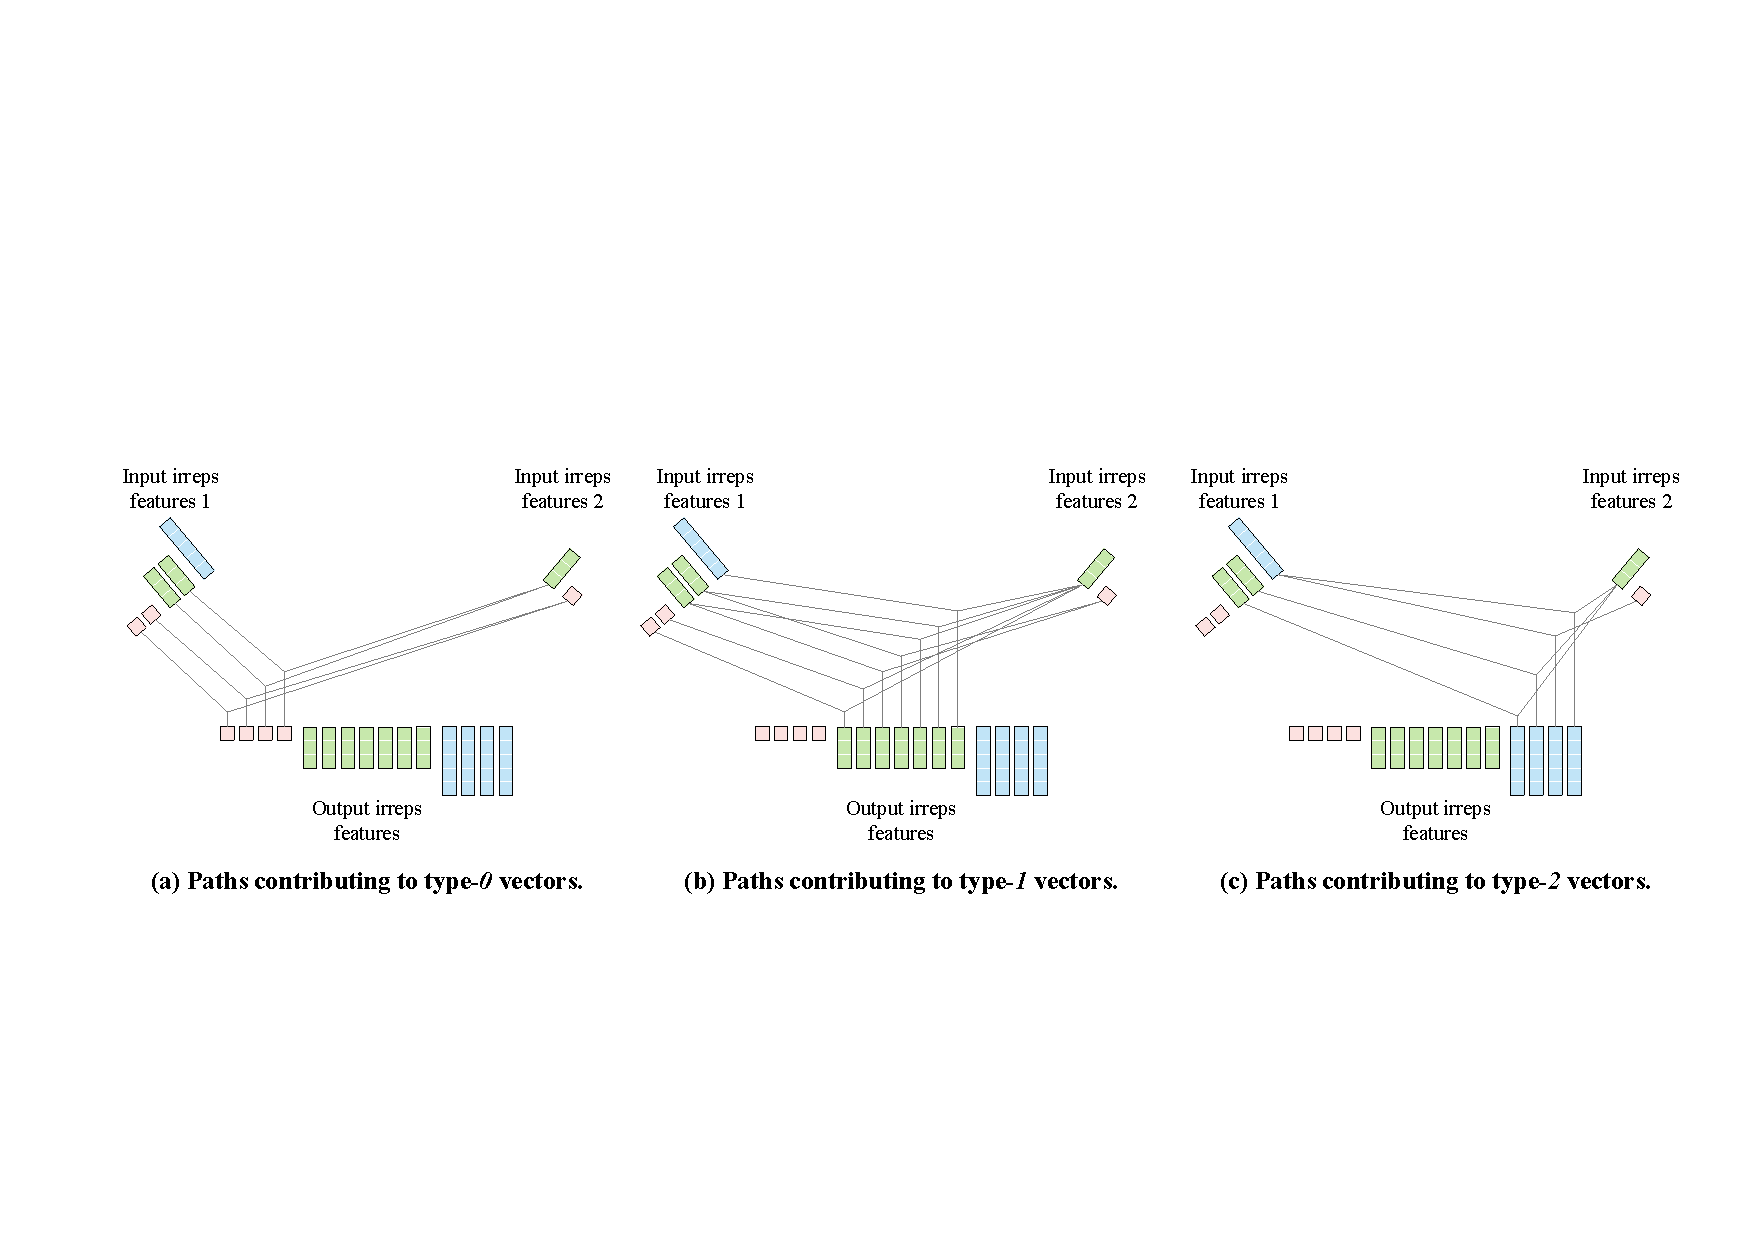
\includegraphics[width=0.99\linewidth]{figure/depthwise_tensor_product_e3nn.pdf}
\centering
\caption{\textbf{An alternative visualization of the depth-wise tensor product. }
We follow the visualization of tensor products in \texttt{e3nn}~\citep{e3nn} and separate paths into three parts based on the types of output vectors.
We note that one vector in the output irreps feature depends only on one vector in each input irreps feature.
}
\label{fig:depthwise_tensor_product_e3nn}
\end{figure*}



\begin{figure*}[th]
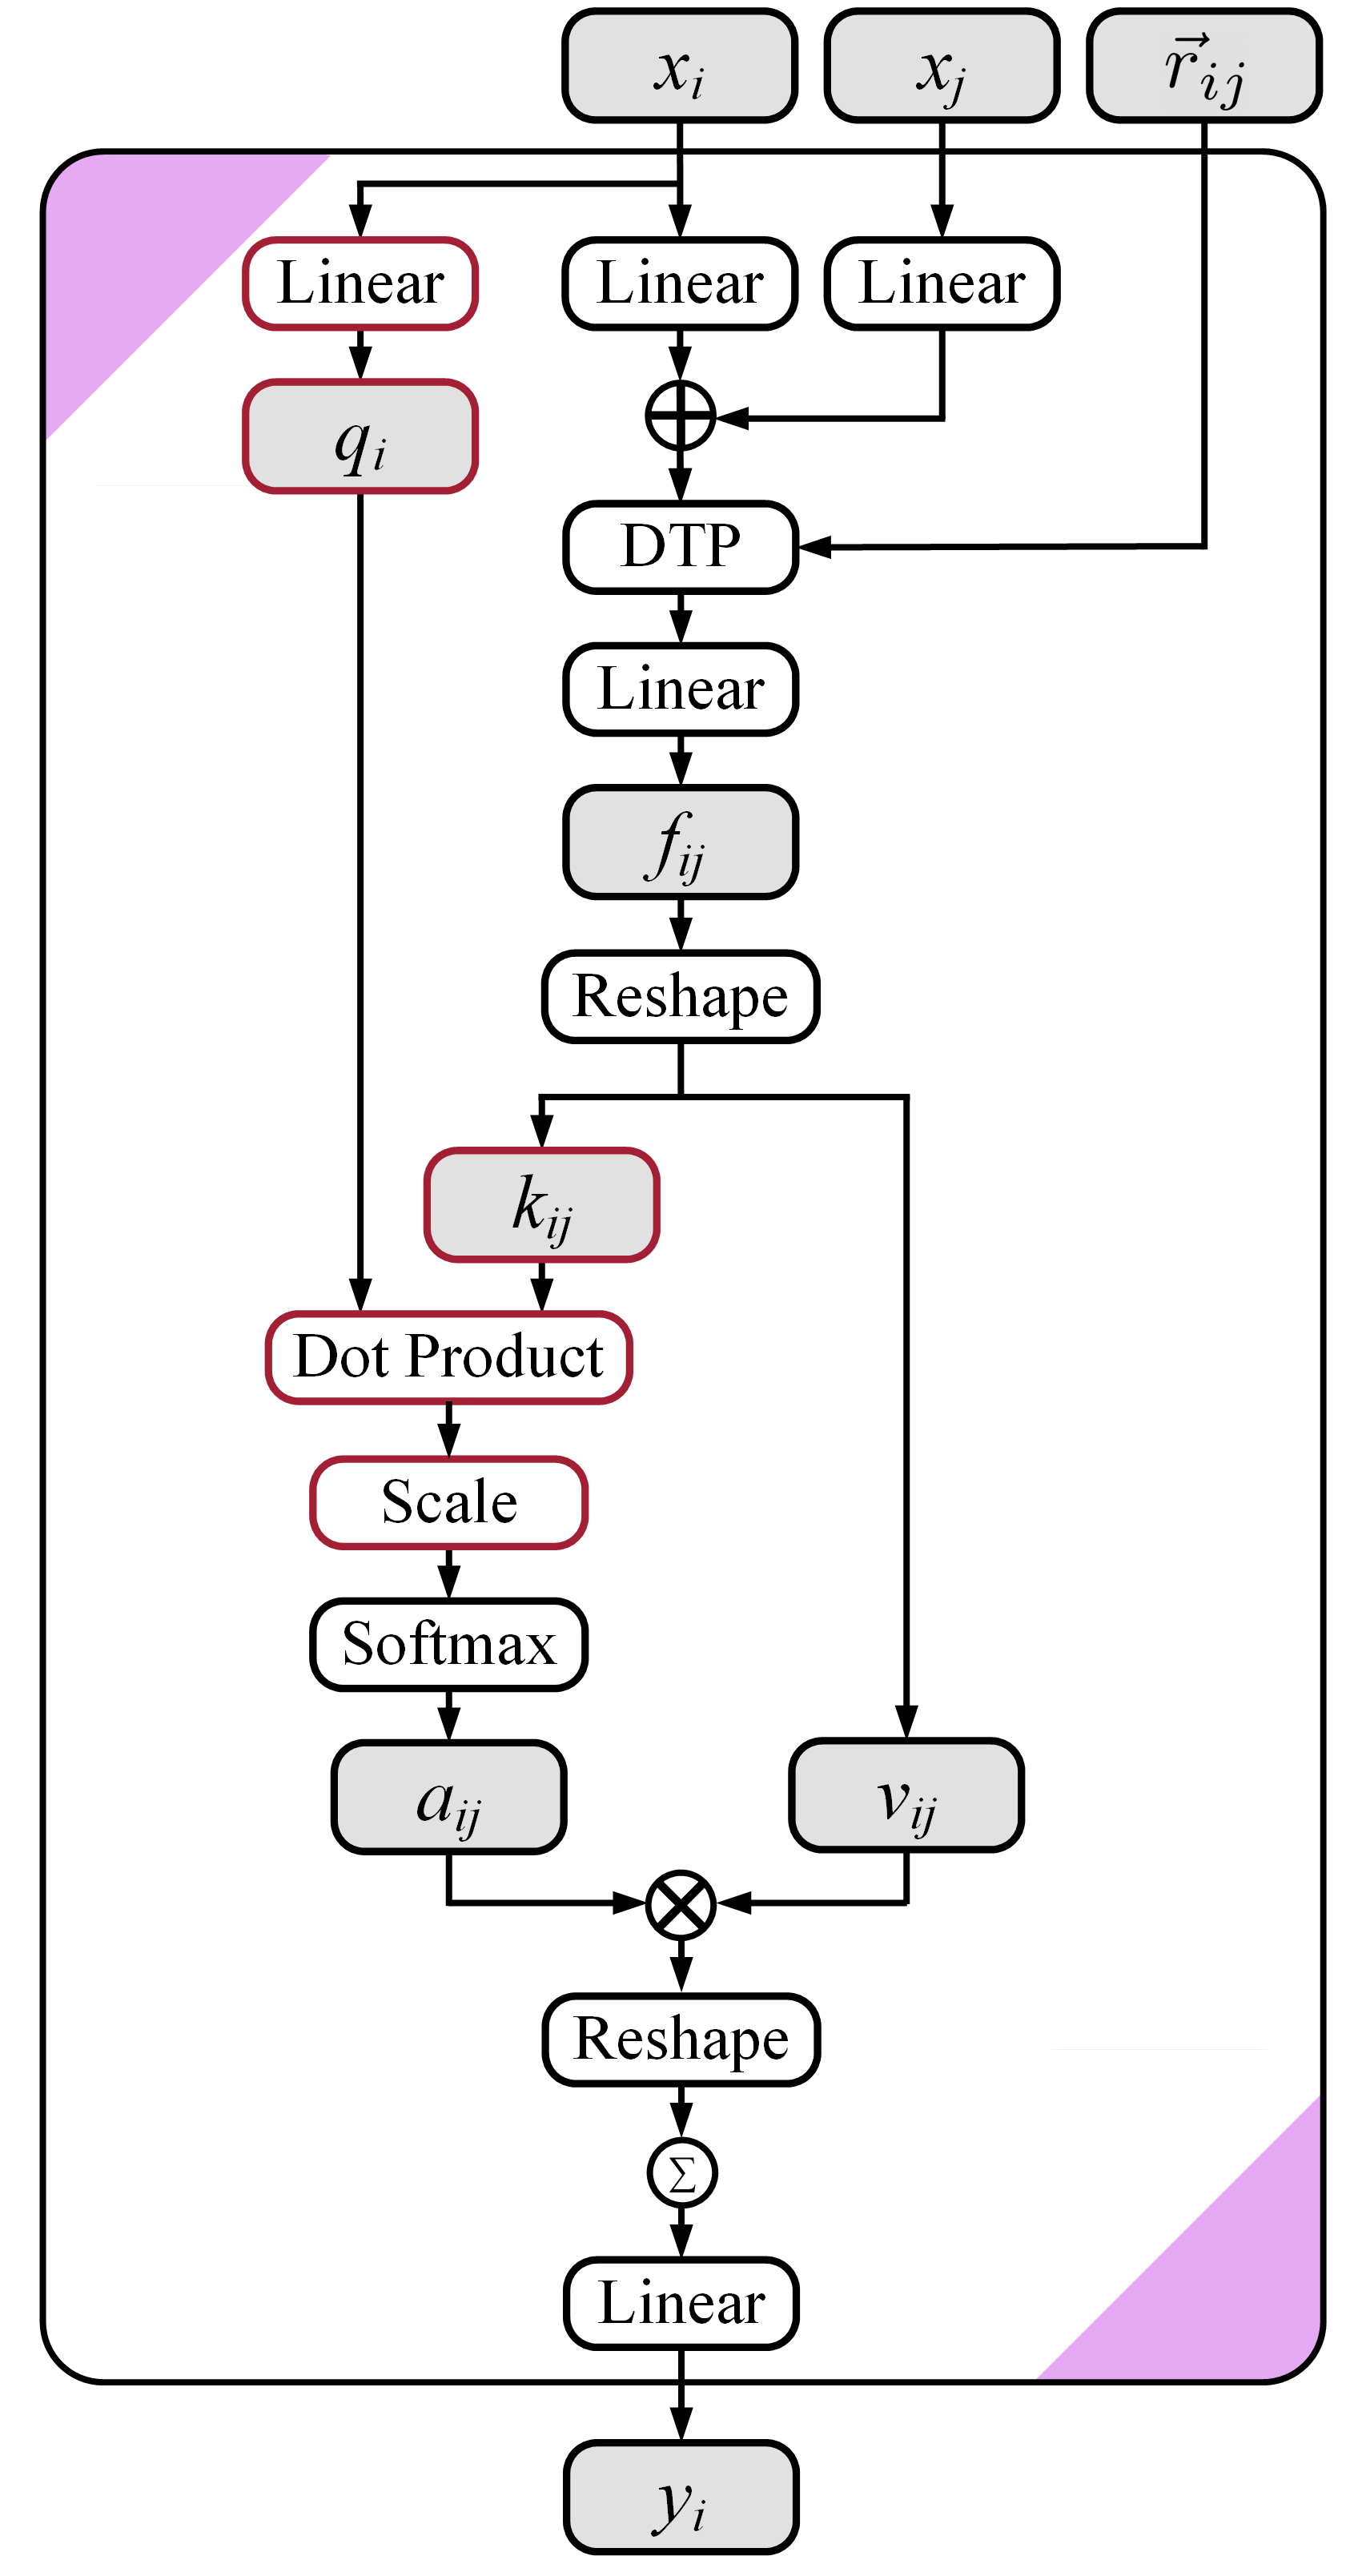
\includegraphics[width=0.35\linewidth]{figure/dot_product_attention.png}
\centering
\caption{\textbf{Architecture of equivariant dot product attention without non-linear message passing.}
In this figure, ``$\otimes$'' denotes multiplication, ``$\oplus$'' denotes addition, and ``DTP'' stands for depth-wise tensor product. $\sum$ within a circle denotes summation over all neighbors.
Gray cells indicate intermediate irreps features.
We highlight the difference of dot product attention from multi-layer perceptron attention in \note{red}.
Note that key $k_{ij}$ and value $v_{ij}$ are irreps features and therefore $f_{ij}$ in dot product attention typically has more channels than that in multi-layer perceptron attention.
}
\label{appendix:fig:dot_product_attention}
\end{figure*}



\subsection{Equivariant Operation Used in Equiformer}
\label{appendix:subsec:equivariant_operations}
We illustrate the equivariant operations used in Equiformer in Fig.~\ref{fig:equivariant_operation} and provide an alternative visualization of depth-wise tensor products in Fig.~\ref{fig:depthwise_tensor_product_e3nn}.

\revision{Besides, we analyze how each equivariant operation remains equivariant and satisfies that $f(D_X(g) x) = D_Y(g) f(x)$, where $f$ is a function mapping between vector spaces $X$ and $Y$, and $D_X(g)$ and $D_Y(g)$ are transformation matrices parametrized by $g$ in $X$ and $Y$.}
\revision{
\begin{enumerate}
    \item \textbf{Linear.} Since for each degree $L$, one output type-$L$ vector is a linear combination of other input type-$L$ vectors, which are transformed by the same matrix $D_X(g)$, the output type-$L$ vector is transformed by the same matrix, meaning that $D_X(g) = D_Y(g)$. 
    \item \textbf{Layer normalization.} For scalar parts ($L = 0$), they are always the same regardless of $E(3)$ transformations, and thus we can apply any function to them. For non-scalar parts ($L > 0$), the L2-norm of any type-$L$ vector is invariant to $E(3)$ transformations. Therefore, the scaling of dividing by the root mean square value (RMS) of L2-norm and multiplying by a learnable parameter $\gamma$ remains the same under $E(3)$ transformations. Multiplying an equivariant feature with an invariant number results in an equivariant feature, and therefore the operation is equivariant. 
    \item \textbf{Gate.} Similar to layer normalization, we can apply any function to the scalar part ($L = 0$). We apply SiLU to the first $C_0$ channels of the scalar part and sigmoid to other channels to obtain non-linear weights. For the non-scalar part ($L > 0$), we multiply each type-$L$ vector with its corresponding non-linear weight. Since the non-linear weights are invariant, multiplying equivariant features with those non-linear weights results in equivariant features.
    \item \textbf{Depth-wise tensor product.} This operation is based on equivariant tensor product operations and restricts that one channel in output irreps feature depends on one channel in input irreps features. The one-to-one dependence of channels does not change the interaction of different type-$L$ vectors, and therefore, the operation is equivariant.
\end{enumerate}
}


\subsection{Equiformer Architecture}
\label{appendix:subsec:equiformer_architecture}

%\todo{Spherical harmonics embeddings}

%\revision{For efficiency and because most works we compare with do not include equivariance to inversion, we mainly adopt $SE(3)$-equivariant irreps features in Equiformer for experiments and note that we can easily incorporate $E(3)$-equivariant irreps features.}
For simplicity and because most works we compare with do not include equivariance to inversion, we adopt $SE(3)$-equivariant irreps features in Equiformer for experiments in the main text and note that $E(3)$-equivariant irreps features can be easily incorporated into Equiformer.
%For clarity, we denote Equiformer with $SE(3)$-equivariant features as ``Equiformer'' and Equiformer with $E(3)$-equivariant features as ``$E(3)$-Equiformer''.

We define architectural hyper-parameters like the number of channels in some layers in Equiformer, which are used to specify the detailed architectures in Sec.~\ref{appendix:subsec:qm9_training_details}, Sec.~\ref{appendix:subsec:md17_training_details} and Sec.~\ref{appendix:subsec:oc20_training_details}.

We use $d_{embed}$ to denote embedding dimension, which defines the dimension of most irreps features.
%Specifically, all irreps features $x_i, y_i$ in Fig.~\ref{fig:equiformer} have dimension $d_{embed}$ unless otherwise stated.
Specifically, all irreps features $x_i, y_i$ in Fig.~\ref{fig:equiformer} have dimension $d_{embed}$ unless otherwise stated.
Besides, we use $d_{sh}$ to represent the dimension of spherical harmonics embeddings of relative positions in all depth-wise tensor products.

%For equivariant graph attention in Fig.~\ref{fig:equiformer}(b), the first two linear layers have the same output dimension $d_{embed}$.
For equivariant graph attention in Fig.~\ref{fig:equiformer}(b), the first two linear layers have the same output dimension $d_{embed}$.
The output dimension of depth-wise tensor products (DTP) are determined by that of input irreps features.
Equivariant graph attention consists of $h$ parallel attention functions, and the value vector in each attention function has dimension $d_{head}$.
We refer to $h$ and $d_{head}$ as the number of heads and head dimension, respectively.
By default, we set the number of channels in scalar feature $f_{ij}^{(0)}$ to be the same as the number of channels of type-$0$ or type-$(0, e)$ vectors in $v_{ij}$.
When non-linear messages are adopted in $v_{ij}$, we set the dimension of output irreps features in gate activation to be $h \times d_{head}$.
Therefore, we can use two hyper-parameters $h$ and $d_{head}$ to specify the detailed architecture of equivariant graph attention.

As for feed forward networks (FFNs), we denote the dimension of output irreps features in gate activation as $d_{ffn}$.
The FFN in the last Transformer block has output dimension $d_{feature}$, and we set $d_{ffn}$ of the last FFN, which is followed by output head, to be $d_{feature}$ as well.
Thus, two hyper-parameters $d_{ffn}$ and $d_{feature}$ are used to specify architectures of FFNs and the output dimension after Transformer blocks.

Irreps features contain channels of vectors with degrees up to $L_{max}$.
We denote $C_L$ type-$L$ vectors as $(C_L, L)$ and $C_{(L, p)}$ type-$(L, p)$ vectors as $(C_{(L, p)}, L, p)$ and use brackets to represent concatenations of vectors.
For example, the dimension of irreps features containing $256$ type-$0$ vectors and $128$ type-$1$ vectors can be represented as $[(256, 0), (128, 1)]$.
%We can extend this to include inversion by introducing parity $p$ and using $(C_{(L, p)}, L, p)$.







\subsection{Dot Product Attention}
\label{appendix:subsec:dot_product_attention}
%We illustrate the dot product attention without non-linear message passing used in ablation study in Fig.~\ref{fig:dot_product_attention}.
We illustrate the dot product attention without non-linear message passing used in ablation study in Fig.~\ref{appendix:fig:dot_product_attention}.
The architecture is adapted from SE(3)-Transformer~\citep{se3_transformer}.
The difference from multi-layer perceptron attention lies in how we obtain attention weights $a_{ij}$ from $f_{ij}$.
We split $f_{ij}$ into two irreps features, key $k_{ij}$ and value $v_{ij}$, and obtain query $q_{i}$ with a linear layer.
Then, we perform scaled dot product~\citep{transformer} between $q_i$ and $k_{ij}$ for attention weights.


\subsection{\revision{Incorporating $E(3)$-Equivariance}}
\label{appendix:subsec:incorporating_e3_equivariance}
\revision{To incorporate $E(3)$-equivariance to Equiformer, we can directly use the same architecture described in Fig.~\ref{fig:equiformer} with the following two modifications:}
\revision{
\begin{enumerate}
    \item We change internal representations from type-$L$ vectors to type-$(L, p)$ vectors as mentioned in Sec.~\ref{appendix:subsec:equivariant_irreps_feature}. Note that type-$(L, e)$ vectors and type-$(L, o)$ vectors are considered different types by equivariant operations and that scalars correspond to only type-$(0, e)$ vectors and do not include type-$(0, o)$ vectors. 
    \item The behaviors of equivariant operations are changed accordingly since parities $p$ are included in internal representations. 
    The operations of linear and layer normalization will treat type-$(L, e)$ vectors and type-$(L, o)$ vectors as different types. 
    This means that we linearly combine or normalize these two types of vectors in a separate manner. 
    In Sec.~\ref{appendix:subsec:tensor_product}, we discuss how tensor products behave when $E(3)$ equivariance is considered. 
    For the operation of gate, we apply activation functions to type-$(0, e)$ vectors (scalars) and treat type-$(0, o)$ vectors (pseudo-scalars) in the same manner as vectors of higher $L$. 
    Specifically, given input $x$ containing non-scalar $C_{(L, p)}$ type-$(L, p)$ vectors with $0 < L \leq L_{max}$ and $p \in \{e, o\}$, $C_{(0, o)}$ type-$(0, o)$ vectors and $(C_{(0, e)} + C_{(0, o)} + \sum_{L=1}^{L_{max}} \sum_{p \in \{e, o\}}C_{(L, p)})$ type-$(0, e)$ vectors, we apply SiLU to the first $C_{(0, e)}$ type-$(0, e)$ vectors and sigmoid function to the other $( C_{(0, o)} + \sum_{L=1}^{L_{max}} \sum_{p \in \{e, o\}}C_{(L, p)})$ type-$(0, e)$ vectors to obtain non-linear weights and multiply each pseudo-scalar or type-$(L, p)$ vector with corresponding non-linear weights. After the gate activation, the number of channels for type-$(0, e)$ vectors is reduced to $C_{(0, e)}$.  
\end{enumerate}
}
\revision{}

\subsection{Discussion on Computational Complexity}
\label{appendix:subsec:computational_complexity}


We discuss the computational complexity of the proposed equivariant graph attention here.

First, we compare dot product attention with MLP attention when linear messages are used for value $v_{ij}$.
Dot product attention requires taking the dot product of two irreps features, query $q_i$ and key $k_{ij}$, for attention weights, and both $q_i$ and $k_{ij}$ have the same dimension as value $v_{ij}$.
In contrast, MLP attention uses only scalar features $f_{ij}^{(0)}$ for attention weights.
The dimension of scalar features $f_{ij}^{(0)}$ is the same as that of the scalar part of $v_{ij}$.
Therefore, MLP attention generates less and smaller intermediate features for attention weights and is faster than dot product attention.

Second, compared to linear messages, using non-linear messages increases the number of tensor product operations from $1$ to $2$.
Since tensor products are compute-intensive, this inevitably increases training and inference time.

Please refer to Sec.~\ref{appendix:subsec:qm9_training_details} and Sec.~\ref{appendix:subsec:oc20_training_details} for the exact numbers of training time on QM9 and OC20.
\section{Details of Experiments on QM9}
\label{appendix:sec:qm9}



\begin{table}[]
\centering
\resizebox{\ifdim\width>\textwidth\textwidth\else\width\fi}{!}{
\begin{tabular}{ll}
%\cline{7-11}
\toprule[1.2pt]
Hyper-parameters & Value or description
 \\
\midrule[1.2pt]
Optimizer & AdamW \\
Learning rate scheduling & Cosine learning rate with linear warmup \\
Warmup epochs & $5$ \\
%Maximum learning rate & $1.5 \times 10 ^{-4}$ for $G$, $H$, $U$ and $U_0$, and $5 \times 10 ^{-4}$ for others \\
Maximum learning rate & $1.5 \times 10 ^{-4}$, $5 \times 10 ^{-4}$ \\
%Batch size & $64$ for $G$, $H$, $U$ and $U_0$, and $128$ for others \\
Batch size & $64$, $128$ \\
%Number of epochs & $600$ for $G$, $H$, $U$ and $U_0$, and $300$ for others \\
Number of epochs & $300$, $600$ \\
%Weight decay & $0$ for $G$, $H$, $U$ and $U_0$, and $5 \times 10^{-3}$ for others \\
Weight decay & $0$, $5 \times 10^{-3}$ \\
%Dropout rate & $0.0$ for $G$, $H$, $U$ and $U_0$, $0.1$ for $R^{2}$, and $0.2$ for others \\
Dropout rate & $0.0$, $0.1$, $0.2$ \\
% ===============================
%   Add this back in the futrure
% ===============================
%Dropout rate & $0.1$, $0.2$ \\
\midrule[0.6pt]
Cutoff radius ($\angstrom$) & $5$ \\
Number of radial bases & $128$ for Gaussian radial basis, $8$ for radial bessel basis \\
Hidden sizes of radial functions & $64$ \\
Number of hidden layers in radial functions & $2$ \\

\midrule[0.6pt]

\multicolumn{2}{c}{Equiformer} \\
\\
Number of Transformer blocks & $6$ \\
Embedding dimension $d_{embed}$ & $[(128, 0), (64, 1), (32, 2)]$ \\
Spherical harmonics embedding dimension $d_{sh}$ & $[(1, 0), (1, 1), (1, 2)]$ \\
Number of attention heads $h$ & $4$ \\
Attention head dimension $d_{head}$ & $[(32, 0), (16, 1), (8, 2)]$\\
Hidden dimension in feed forward networks $d_{ffn}$ & $[(384, 0), (192, 1) , (96, 2)]$ \\
Output feature dimension $d_{feature}$ & $[(512, 0)]$\\

\midrule[0.6pt]

\multicolumn{2}{c}{$E(3)$-Equiformer} \\
\\
Number of Transformer blocks & $6$ \\
Embedding dimension $d_{embed}$ & $[(128, 0, e), (32, 0, o), (32, 1, e), (32, 1, o), (16, 2, e), (16, 2, o)]$ \\
Spherical harmonics embedding dimension $d_{sh}$ & $[(1, 0, e), (1, 1, o), (1, 2, e)]$ \\
Number of attention heads $h$ & $4$ \\
Attention head dimension $d_{head}$ & $[(32, 0, e), (8, 0, o), (8, 1, e), (8, 1, o), (4, 2, e), (4, 2, o)]$ \\
Hidden dimension in feed forward networks $d_{ffn}$ & $[(384, 0, e), (96, 0, o), (96, 1, e), (96, 1, o), (48, 2, e), (48, 2, o)]$ \\
Output feature dimension $d_{feature}$ & $[(512, 0, e)]$\\
\bottomrule[1.2pt]
\end{tabular}
}
\vspace{-2mm}
\caption{\textbf{Hyper-parameters for QM9 dataset.}
We denote $C_L$ type-$L$ vectors as $(C_L, L)$ and $C_{(L, p)}$ type-$(L, p)$ vectors as $(C_{(L, p)}, L, p)$ and use brackets to represent concatenations of vectors.
}
\label{appendix:tab:qm9}
\end{table}


\subsection{Training Details}
\label{appendix:subsec:qm9_training_details}
%%%We normalize ground truth by subtracting mean and dividing by standard deviation.
%%%For the task of $U$, $U_0$, $G$, and $H$, where single-atom reference values are available, we subtract those reference values from ground truth before normalizing. 
We use the same data partition as TorchMD-NET~\citep{torchmd_net}.
For the task of $U$, $U_0$, $G$, and $H$, where single-atom reference values are available, we subtract those reference values from ground truth. 
For other tasks, we normalize ground truth by subtracting mean and dividing by standard deviation.

We train Equiformer with 6 blocks with $L_{max} = 2$.
%We choose Gaussian radial basis~\cite{schnet, spinconv, gemnet, graphormer_3d} for the first six tasks in Table~\ref{tab:qm9_result} and radial Bessel basis for the others.
We choose Gaussian radial basis~\citep{schnet, spinconv, gemnet, graphormer_3d} for the first six tasks in Table~\ref{tab:qm9_result} and radial Bessel basis~\citep{dimenet, dimenet_pp} for the others.
% ===============================
%   Add these back in the future
% ===============================
We apply dropout~\citep{dropout} to attention weights $a_{ij}$.
The dropout rate is $0.0$ for the tasks of $G$, $H$, $U$ and $U_0$, is $0.1$ for the task of $R^2$ and is $0.2$ for others.
Since the tasks of $G$, $H$, $U$, and $U_0$ require longer training, we use slightly different hyper-parameters.
The number of epochs is $600$ for the tasks of $G$, $H$, $U$, and $U_0$ and is $300$ for others.
The learning rate is $1.5 \times 10 ^{-4}$ for the tasks of $G$, $H$, $U$, and $U_0$ and is $5 \times 10^{-4}$ for others.
The batch size is $64$ for the tasks of $G$, $H$, $U$, and $U_0$ and is $128$ for others.
The weight decay is $0$ for the tasks of $G$, $H$, $U$, and $U_0$ and is $5 \times 10^{-3}$ for others.
Table~\ref{appendix:tab:qm9} summarizes the hyper-parameters for the QM9 dataset.
The detailed description of architectural hyper-parameters can be found in Sec.~\ref{appendix:subsec:equiformer_architecture}. 

We use one A6000 GPU with 48GB to train each model and summarize the computational cost of training for one epoch as follows.
Training $E(3)$-Equiformer in Table~\ref{appendix:tab:e3_qm9} for one epoch takes about $16.3$ minutes.
The time of training Equiformer, Equiformer with linear messages (indicated by Index $2$ in Table~\ref{tab:qm9_ablation}), and Equiformer with linear messages and dot product attention (indicated by Index $3$ in Table~\ref{tab:qm9_ablation}) for one epoch is $12.1$ minutes, $7.2$ minutes and $7.8$ minutes, respectively.


%We set cutoff radius to be $5 \angstrom$ and represent relative distances with Gaussian radial basis~\cite{schnet, spinconv, gemnet, graphormer_3d} with dimension $128$.
%Please refer to appendix for further details on Equiformer architecture.
%\todo{We apply dropout~\cite{dropout} with probability $0.2$ to attention weights}. 
%We use AdamW optimizer~\cite{adamw} with weight decay $5 \times 10^{-3}$ and use cosine learning rate with linear warmup, where the maximum learning rate is $5 \times 10 ^{-4}$ and warmup epoch is $5$.
%The batch size is $128$ and the number of epochs is $300$.


\subsection{Comparison between $SE(3)$ and $E(3)$ Equivariance}
\label{appendix:subsec:e3_qm9}
We train two versions of Equiformers, one with $SE(3)$-equivariant features denoted as ``Equiformer'' and the other with $E(3)$-equivariant features denoted as ``$E(3)$-Equiformer'', and we compare them in Table~\ref{appendix:tab:e3_qm9}.
%Including equivariance to inversion further improves the performance on QM9 dataset.
As for Table~\ref{tab:qm9_result}, we compare ``Equiformer'' with other works since most of them do not include equivariance to inversion.

\begin{table}[th]
\centering
\resizebox{\ifdim\width>\textwidth\textwidth\else\width\fi}{!}{
\begin{tabular}{llccccccccc}
%\cline{7-11}
\toprule[1.2pt]
& Task & $\alpha$ & $\Delta \varepsilon$ & $\varepsilon_{\text{HOMO}}$ & $\varepsilon_{\text{LUMO}}$ & $\mu$ & $C_{\nu}$ & Training time & Number of \\
%Methods & Units & bohr$^3$ & meV & meV & meV & D & cal/mol K & (minutes/epoch) & parameters \\
Methods & Units & $a_0^3$ & meV & meV & meV & D & cal/mol K & (minutes/epoch) & parameters \\
\midrule[1.2pt]


Equiformer & & .046 & 30 & 15 & 14 & .011 & .023 & 12.1 & 3.53M \\
$E(3)$-Equiformer & & .045 & 30 & 15 & 14 & .012 & .023 & 16.3 & 3.28M\\
%\midrule[0.6pt]
%Equiformer + NAT & 0.4737 & 0.7245 & 0.4862 & 0.6493 & 0.5834 & 6.01 & 2.45 & 5.41 & 2.71 & \\
\bottomrule[1.2pt]

\end{tabular}
}
\vspace{-2mm}
\caption{\textbf{Ablation study of $SE(3)$/$E(3)$ equivariance on QM9 testing set.}  
``Equiformer'' operates on $SE(3)$-equivariant features while ``$E(3)$-Equiformer'' uses $E(3)$-equivariant features.
Including inversion achieves similar performance.
}
\vspace{-2.5mm}
\label{appendix:tab:e3_qm9}
\end{table}


\subsection{Comparison of Training Time and Numbers of Parameters}
\label{appendix:subsec:qm9_training_time_comparison}
We compare training time and numbers of parameters between SEGNN~\citep{segnn}, TorchMD-NET~\citep{torchmd_net} and Equiformer and summarize the results in Table~\ref{appendix:tab:qm9_training_time}.
Training Equiformer for $300$ epochs and for $600$ epochs takes $61$ and $122$ GPU-hours, respectively.

Compared to SEGNN, which is written with the same \texttt{e3nn} library~\citep{e3nn}, Equiformer with MLP attention and non-linear message is faster.
Although Equiformer has more channels and more parameters, the training time is comparable. 
The reasons are as follows.
Equiformer uses more efficient depth-wise tensor products (DTP), where one output channel depends on only one input channel. 
SEGNN uses more compute-intensive fully connected tensor products (FCTP), where one output channel depends on all input channels. 
Besides, SEGNN uses 4 FCTPs in each message passing block while Equiformer uses only 2 DTPs in each block. 

Compared to TorchMD-NET, which is trained for $3000$ epochs, Equiformer achieves competitve results after trained for $300$ or $600$ epochs.
Equiformer takes more time for each epoch since Equiformer uses more expressive non-linear messages, which compared to linear messages used in other equivariant Transformers, doubles the number of tensor products and therefore almost doubles the training time.
Moreover, Equiformer incorporates tensors of higher degrees (e.g., $L_{max}=2$), which improves performance but slows down the training.



\begin{table}[t]
\begin{adjustwidth}{0cm}{0cm}
\centering
\resizebox{\ifdim\width>\textwidth\textwidth\else\width\fi}{!}{
\begin{tabular}{lccc}
%\cline{7-11}
\toprule[1.2pt]
Methods & Number of parameters & Training time (GPU-hours) \\
\midrule[1.2pt]

SEGNN~\citep{segnn} & 1.03M & 81 \\
TorchMD-NET~\citep{torchmd_net} & 6.86M & 92 \\
\midrule[0.6pt]
Equiformer & 3.53M & 61 \\

\bottomrule[1.2pt]

\end{tabular}
}
\vspace{-3mm}
\end{adjustwidth}
\caption{\textbf{Comparison of training time and numbers of parameters for QM9 dataset.}  
%\note{Dropout rate = 0.1.}
%%%$\dagger$ denotes using different training, validation, testing data partitions. % as mentioned in SEGNN~\cite{segnn}.
%$\dagger$ denotes using different data partitions.
%$\ddagger$ denotes results from SE(3)-Transformer~\cite{se3_transformer}.
}
\label{appendix:tab:qm9_training_time}
\end{table}
\section{Details of Experiments on MD17}
\label{appendix:sec:md17}


\subsection{Training Details}
\label{appendix:subsec:md17_training_details}
%%%We normalize ground truth by subtracting mean and dividing by standard deviation.
%%%For the task of $U$, $U_0$, $G$, and $H$, where single-atom reference values are available, we subtract those reference values from ground truth before normalizing. 
%We use the same data partition as TorchMD-NET~\citep{torchmd_net}.
%For the task of $U$, $U_0$, $G$, and $H$, where single-atom reference values are available, we subtract those reference values from ground truth. 
%For other tasks, we normalize ground truth by subtracting mean and dividing by standard deviation.

We use the same data partition as TorchMD-NET~\citep{torchmd_net}.
For energy prediction, we normalize ground truth by subtracting mean and dividing by standard deviation.
For force prediction, we normalize ground truth by dividing by standard deviation of ground truth energy.

We train Equiformer with 6 blocks with $L_{max} = 2 \text{ and } 3$.
%We choose Gaussian radial basis~\cite{schnet, spinconv, gemnet, graphormer_3d} for the first six tasks in Table~\ref{tab:qm9_result} and radial Bessel basis for the others.
We choose the radial basis function used by PhysNet~\citep{physnet}.
We do not apply dropout to attention weights $a_{ij}$.
For Equiformer with $L_{max} = 2$, the learning rate is $1 \times 10 ^{-4}$ for benzene and is $5 \times 10^{-4}$ for others. 
The batch size is $8$, and the number of epochs is $1500$.
The model has about $3.50$M parameters.
For Equiformer with $L_{max} = 3$, the learning rate is $1 \times 10 ^{-4}$ for benzene and is $2 \times 10^{-4}$ for others. 
The batch size is $5$, and the number of epochs is $2000$.
The model has about $5.50$M parameters.
%The dropout rate is $0.0$ for the tasks of $G$, $H$, $U$ and $U_0$, is $0.1$ for the task of $R^2$ and is $0.2$ for others.
%Since the tasks of $G$, $H$, $U$, and $U_0$ require longer training, we use slightly different hyper-parameters.
%The number of epochs is $600$ for the tasks of $G$, $H$, $U$, and $U_0$ and is $300$ for others.
%The learning rate is $1.5 \times 10 ^{-4}$ for the tasks of $G$, $H$, $U$, and $U_0$ and is $5 \times 10^{-4}$ for others.
%The batch size is $64$ for the tasks of $G$, $H$, $U$, and $U_0$ and is $128$ for others.
%The weight decay is $0$ for the tasks of $G$, $H$, $U$, and $U_0$ and is $5 \times 10^{-3}$ for others.
Table~\ref{appendix:tab:md17} summarizes the hyper-parameters for the MD17 dataset.
The detailed description of architectural hyper-parameters can be found in Sec.~\ref{appendix:subsec:equiformer_architecture}. 

We use one A5000 GPU with 24GB to train different models for each molecule.
%Each model takes about $26.5$ hours.
Training Equiformer with $L_{max} = 2$ takes about $15.4$ hours, and training Equiformer with $L_{max} = 3$ takes about $54.4$ hours.

\begin{table}[]
\centering
\resizebox{\ifdim\width>\textwidth\textwidth\else\width\fi}{!}{
\begin{tabular}{ll}
%\cline{7-11}
\toprule[1.2pt]
Hyper-parameters & Value or description
 \\
\midrule[1.2pt]
Optimizer & AdamW \\
Learning rate scheduling & Cosine learning rate with linear warmup \\
Warmup epochs & $10$ \\
%Maximum learning rate & $1.5 \times 10 ^{-4}$ for $G$, $H$, $U$ and $U_0$, and $5 \times 10 ^{-4}$ for others \\
Maximum learning rate & $1 \times 10 ^{-4}$, $2 \times 10^{-4}$, $5 \times 10 ^{-4}$ \\
%Batch size & $64$ for $G$, $H$, $U$ and $U_0$, and $128$ for others \\
Batch size & $5$, $8$ \\
%Number of epochs & $600$ for $G$, $H$, $U$ and $U_0$, and $300$ for others \\
Number of epochs & $1500$, $2000$ \\
%Weight decay & $0$ for $G$, $H$, $U$ and $U_0$, and $5 \times 10^{-3}$ for others \\
Weight decay & $1 \times 10^{-6}$ \\
%Dropout rate & $0.0$ for $G$, $H$, $U$ and $U_0$, $0.1$ for $R^{2}$, and $0.2$ for others \\
Dropout rate & $0.0$ \\
\midrule[0.6pt]
Weight for energy loss & $1$ \\
Weight for force loss & $80$ \\
% ===============================
%   Add this back in the futrure
% ===============================
%Dropout rate & $0.1$, $0.2$ \\
\midrule[0.6pt]
Cutoff radius ($\angstrom$) & $5$ \\
Number of radial bases & $32$ \\
Hidden sizes of radial functions & $64$ \\
Number of hidden layers in radial functions & $2$ \\

\midrule[0.6pt]

\multicolumn{2}{c}{Equiformer ($L_{max} = 2$)} \\
\\
Number of Transformer blocks & $6$ \\
Embedding dimension $d_{embed}$ & $[(128, 0), (64, 1), (32, 2)]$ \\
Spherical harmonics embedding dimension $d_{sh}$ & $[(1, 0), (1, 1), (1, 2)]$ \\
Number of attention heads $h$ & $4$ \\
Attention head dimension $d_{head}$ & $[(32, 0), (16, 1), (8, 2)]$\\
Hidden dimension in feed forward networks $d_{ffn}$ & $[(384, 0), (192, 1) , (96, 2)]$ \\
Output feature dimension $d_{feature}$ & $[(512, 0)]$\\

\midrule[0.6pt]

\multicolumn{2}{c}{Equiformer ($L_{max} = 3$)} \\
\\
Number of Transformer blocks & $6$ \\
Embedding dimension $d_{embed}$ & $[(128, 0), (64, 1), (64, 2), (32, 3)]$ \\
Spherical harmonics embedding dimension $d_{sh}$ & $[(1, 0), (1, 1), (1, 2), (1, 3)]$ \\
Number of attention heads $h$ & $4$ \\
Attention head dimension $d_{head}$ & $[(32, 0), (16, 1), (16, 2), (8, 3)]$\\
Hidden dimension in feed forward networks $d_{ffn}$ & $[(384, 0), (192, 1), (192, 2), (96, 3)]$ \\
Output feature dimension $d_{feature}$ & $[(512, 0)]$\\

%\midrule[0.6pt]

%\multicolumn{2}{c}{$E(3)$-Equiformer} \\
%\\
%Number of Transformer blocks & $6$ \\
%Embedding dimension $d_{embed}$ & $[(128, 0, e), (32, 0, o), (32, 1, e), (32, 1, o), (16, 2, e), (16, 2, o)]$ \\
%Spherical harmonics embedding dimension $d_{sh}$ & $[(1, 0, e), (1, 1, o), (1, 2, e)]$ \\
%Number of attention heads $h$ & $4$ \\
%Attention head dimension $d_{head}$ & $[(32, 0, e), (8, 0, o), (8, 1, e), (8, 1, o), (4, 2, e), (4, 2, o)]$ \\
%Hidden dimension in feed forward networks $d_{ffn}$ & $[(384, 0, e), (96, 0, o), (96, 1, e), (96, 1, o), (48, 2, e), (48, 2, o)]$ \\
%Output feature dimension $d_{feature}$ & $[(512, 0, e)]$\\
\bottomrule[1.2pt]
\end{tabular}
}
\vspace{-2mm}
\caption{\textbf{Hyper-parameters for MD17 dataset.}
We denote $C_L$ type-$L$ vectors as $(C_L, L)$ and $C_{(L, p)}$ type-$(L, p)$ vectors as $(C_{(L, p)}, L, p)$ and use brackets to represent concatenations of vectors.
}
\label{appendix:tab:md17}
\end{table}


\subsection{Additional Comparison to TorchMD-NET}
\label{appendix:subsec:md17_torchmdnet}
Since TorchMD-NET~\citep{torchmd_net} is also an equivariant Transformer but  uses dot product attention instead of the proposed equivariant graph attention, we provide additional comparisons in Table~\ref{appendix:tab:md17_torchmdnet}.
For each molecule, we adjust the ratio of the weight for force loss to the weight for energy loss so that Equiformer with $L_{max} = 2$ can achieve lower MAE for both energy and forces.



\begin{table}[t]
\begin{adjustwidth}{0cm}{0cm}
\centering
\resizebox{\ifdim\width>\textwidth\textwidth\else\width\fi}{!}{
\begin{tabular}{lcccccccccccccccc}
\toprule[1.2pt]
                        & \multicolumn{2}{c}{Aspirin} & \multicolumn{2}{c}{Benzene} & \multicolumn{2}{c}{Ethanol} & \multicolumn{2}{c}{Malonaldehyde} & \multicolumn{2}{c}{Naphthalene} & \multicolumn{2}{c}{Salicylic acid} & \multicolumn{2}{c}{Toluene} & \multicolumn{2}{c}{Uracil} \\
\cmidrule[0.6pt]{2-17}
Methods                                               & energy       & forces       & energy       & forces       & energy       & forces       & energy          & forces          & energy         & forces         & energy           & forces          & energy       & forces       & energy       & forces      \\
\midrule[1.2pt]
%SchNet~\citep{schnet}                          & 16.0         & 58.5         & 3.5          & 13.4         & 3.5          & 16.9         & 5.6             & 28.6            & 6.9            & 25.2           & 8.7              & 36.9            & 5.2          & 24.7         & 6.1          & 24.3        \\
%DimeNet~\citep{dimenet}                          & 8.8          & 21.6         & 3.4          & 8.1          & 2.8          & 10.0         & 4.5             & 16.6            & 5.3            & 9.3            & 5.8              & 16.2            & 4.4          & 9.4          & 5.0          & 13.1        \\
%PaiNN~\citep{painn}                                                 & 6.9          & 14.7         & -            & -            & 2.7          & 9.7          & 3.9             & 13.8            & 5.0            & 3.3            & 4.9              & 8.5             & 4.1          & 4.1          & 4.5          & 6.0         \\
TorchMD-NET                                           & \textbf{5.3}          & 11.0         & 2.5          & 8.5          & 2.3          & 4.7          & 3.3             & 7.3             & \textbf{3.7}            & 2.6            & \textbf{4.0}              & 5.6             & \textbf{3.2}          & 2.9          & \textbf{4.1}          & 4.1         \\
%NequIP ($L_{max} = 3$)~\citep{nequip}                              & 5.7          & 8.0          & -            & -            & \textbf{2.2}          & \textbf{3.1}          & \textbf{3.3}             & \textbf{5.6}             & 4.9            & \textbf{1.7}            & 4.6              & \textbf{3.9}             & 4.0          & \textbf{2.0}          & 4.5          & \textbf{3.3}         \\

\midrule[0.6pt]

Equiformer ($L_{max} = 2$)                                           & \textbf{5.3}          & \textbf{7.2}          & \textbf{2.2}          & \textbf{6.6}          & \textbf{2.2}          & \textbf{3.1}          & \textbf{3.3}             & \textbf{5.8}             & \textbf{3.7}            & \textbf{2.1}           & \textbf{4.0}              & \textbf{5.3}             & \textbf{3.2}         & \textbf{2.4}          & 4.2          & \textbf{3.7}        \\
\bottomrule[1.2pt]
\end{tabular}
}
\end{adjustwidth}
\vspace{-2mm}
\caption{\textbf{Additional comparison to TorchMD-Net~\citep{torchmd_net} on MD17 dataset.} Energy and force are in units of meV and meV/$\angstrom$.}
\label{appendix:tab:md17_torchmdnet}
\end{table}


\subsection{Comparison of Training Time and Numbers of Parameters}
\label{appendix:subsec:md17_training_time_comparison}
We compare training time and number of parameters between NequIP~\citep{nequip} and Equiformer and summarize the results in Table~\ref{appendix:tab:md17_training_time}.
Since NequIP does not report the number of epochs, we compare the time spent for each epoch and note that NequIP is trained for more than $1000$ epochs.
%Equiformer with $L_{max} = 2$ is faster and achieves better MAE results.
Equiformer with $L_{max} = 2$ is faster than NequIP with $L_{max} = 3$ since smaller $L_{max}$ is used.
Moreover, Equiformer with $L_{max} = 2$ achieves overall better results as we use equivariant graph attention instead of linear convolution used by NequIP.
When increasing $L_{max}$ from $2$ to $3$, Equiformer achieves better results than NequIP for most molecules.
However, the training time is longer than NequIP since we use $2$ tensor product operations in each equivariant graph attention instead of $1$ tensor product in each linear convolution.


\begin{table}[t]
\begin{adjustwidth}{0cm}{0cm}
\centering
\resizebox{\ifdim\width>\textwidth\textwidth\else\width\fi}{!}{
\begin{tabular}{lccc}
%\cline{7-11}
\toprule[1.2pt]
Methods & Number of parameters & Training time (secs/epoch) \\
\midrule[1.2pt]

NequIP ($L_{max} = 3$)~\citep{nequip} & 2.97M & 48.7 \\
%TorchMD-NET~\citep{torchmd_net} & 6.9M & 92 \\
\midrule[0.6pt]
Equiformer ($L_{max} = 2$) & 3.50M & 36.9 \\
Equiformer ($L_{max} = 3$) & 5.50M & 98.0 \\

\bottomrule[1.2pt]

\end{tabular}
}
\vspace{-2mm}
\end{adjustwidth}
\caption{\textbf{Comparison of training time and numbers of parameters for MD17 dataset.}  
%\note{Dropout rate = 0.1.}
%%%$\dagger$ denotes using different training, validation, testing data partitions. % as mentioned in SEGNN~\cite{segnn}.
%$\dagger$ denotes using different data partitions.
%$\ddagger$ denotes results from SE(3)-Transformer~\cite{se3_transformer}.
}
\label{appendix:tab:md17_training_time}
\end{table}
\section{Details of Experiments on OC20}
\label{appendix:sec:oc20}


\subsection{Detailed Description of OC20 Dataset}
\label{appendix:subsec:oc20_dataset_details}
The dataset consists of larger atomic systems, each composed of a molecule called adsorbate placed on a slab called catalyst.
Each input contains more atoms and more diverse atom types than QM9 and MD17.
The average number of atoms in a system is more than 70, and there are over 50 atom species.
The goal is to understand interaction between adsorbates and catalysts through relaxation.
%Specifically, an adsorbate is first placed on top of a catalyst at heuristically determined locations in order to form initial structure (IS).
An adsorbate is first placed on top of a catalyst to form initial structure (IS).
The positions of atoms are updated with forces calculated by density function theory until the system is stable and becomes relaxed structure (RS).
The energy of RS, or relaxed energy (RE), is correlated with catalyst activity and therefore a metric for understanding their interaction.
We focus on the task of initial structure to relaxed energy (IS2RE), which predicts relaxed energy (RE) given an initial structure (IS).
%We focus on the task of initial structure to relaxed energy (IS2RE), which is to predict the energy of a relaxed structure (RS) given its initial structure (IS).
There are 460k, 100k and 100k structures in training, validation, and testing sets, respectively.
%%%Performance is measured in MAE and energy within threshold (EwT), the percentage in which predicted energy is within 0.02~eV of ground truth energy.
%%%In validation and testing sets, there are four sub-splits containing in-distribution adsorbates and catalysts (ID), out-of-distribution adsorbates (OOD-Ads), out-of-distribution catalysts (OOD-Cat), and out-of-distribution adsorbates and catalysts (OOD-Both).



\subsection{Training Details}
\label{appendix:subsec:oc20_training_details}
\paragraph{IS2RE without Node-Level Auxiliary Task.}
We use hyper-parameters similar to those for QM9 dataset and summarize in Table~\ref{appendix:tab:oc20}.
For ablation study in Sec.~\ref{subsec:ablation_study}, we use a smaller learning rate $1.5 \times 10 ^{-4}$ for DP attention as this improves the performance.
The detailed description of architectural hyper-parameters can be found in Sec.~\ref{appendix:subsec:equiformer_architecture}. 

%The architecture of Equiformer is the same as that for QM9 except that we use $L_{max} = 1$ and increase numbers of channels.
%Please refer to \todo{appendix} for further details.
%We apply dropout~\cite{dropout} with probability $0.2$ to attention weights. 
%We train models for $20$ epochs with AdamW optimizer~\cite{adamw}, weight decay $1 \times 10^{-3}$, batch size $32$ and cosine learning rate with linear warmup, where the maximum learning rate is $2 \times 10 ^{-4}$ and warmup epoch is $2$.



\paragraph{IS2RE with IS2RS Node-Level Auxiliary Task.}
We increase the number of Transformer blocks to $18$ as deeper networks can benefit more from IS2RS node-level auxiliary task~\citep{noisy_nodes}.
We follow the same hyper-parameters in Table~\ref{appendix:tab:oc20} except that we increase maximum learning rate to $5 \times 10^{-4}$ and set $d_{feature}$ to $[(512, 0), (256, 1)]$.
% ===============================
%   Add these back in the future
% ===============================
%Additionally, we use stochastic depth with probability $0.05$~\cite{drop_path}.
Inspired by Graphormer~\citep{graphormer_3d}, we add an extra equivariant graph attention module after the last layer normalization to predict relaxed structures and use a linearly decayed weight for loss associated with IS2RS, which starts at $15$ and decays to $1$.
For Noisy Nodes~\citep{noisy_nodes} data augmentation, we first interpolate between initial structure and relaxed structure and then add Gaussian noise as described by Noisy Nodes~\citep{noisy_nodes}.
When Noisy Nodes data augmentation is used, we increase the number of epochs to $40$.

We use two A6000 GPUs, each with 48GB, to train models when IS2RS is not included during training.
Training Equiformer and $E(3)$-Equiformer in Table~\ref{appendix:tab:e3_oc20} takes about $43.6$ and $58.3$ hours.
Training Equiformer with linear messages (indicated by Index $2$ in Table~\ref{tab:oc20_ablation}) and Equiformer with linear messages and dot product attention (indicated by Index $3$ in Table~\ref{tab:oc20_ablation}) takes $30.4$ hours and $33.1$ hours, respectively.
We use four A6000 GPUs to train Equiformer models when IS2RS node-level auxiliary task is adopted during training.
Training Equiformer without Noisy Nodes data augmentation takes about $3$ days and training with Noisy Nodes takes $6$ days.
We note that the proposed Equiformer in Table~\ref{tab:is2re_is2rs_testing} achieves competitive results even with much less computation.
Specifically, training ``Equiformer + Noisy Nodes'' takes about $24$ GPU-days when A6000 GPUs are used.
The training time of ``GNS + Noisy Nodes''~\citep{noisy_nodes} is $56$ TPU-days.
``Graphormer''~\citep{graphormer_3d} uses ensemble of $31$ models and requires $372$ GPU-days to train all models when A100 GPUs are used.




\begin{table}[t]
\centering
\resizebox{\ifdim\width>\textwidth\textwidth\else\width\fi}{!}{
\begin{tabular}{ll}
%\cline{7-11}
\toprule[1.2pt]
Hyper-parameters & Value or description
 \\
\midrule[1.2pt]
Optimizer & AdamW \\
Learning rate scheduling & Cosine learning rate with linear warmup \\
Warmup epochs & $2$ \\
Maximum learning rate & $2 \times 10 ^{-4}$ \\
Batch size & $32$ \\
Number of epochs & $20$ \\
Weight decay & $1 \times 10 ^{-3}$\\
Dropout rate & $0.2$ \\
\midrule[0.6pt]
Cutoff radius ($\angstrom$) & $5$ \\
Number of radial basis & $128$ \\
Hidden size of radial function & $64$ \\
Number of hidden layers in radial function & $2$ \\

\midrule[0.6pt]

\multicolumn{2}{c}{Equiformer} \\
\\
Number of Transformer blocks & $6$ \\
Embedding dimension $d_{embed}$ & $[(256, 0), (128, 1)]$ \\
Spherical harmonics embedding dimension $d_{sh}$ & $[(1, 0), (1, 1)]$ \\
Number of attention heads $h$ & $8$ \\
Attention head dimension $d_{head}$ & $[(32, 0), (16, 1)]$\\
Hidden dimension in feed forward networks $d_{ffn}$ & $[(768, 0), (384, 1)]$ \\
Output feature dimension $d_{feature}$ & $[(512, 0)]$\\

\midrule[0.6pt]

\multicolumn{2}{c}{$E(3)$-Equiformer} \\
\\
Number of Transformer blocks & $6$ \\
Embedding dimension $d_{embed}$ & $[(256, 0, e), (64, 0, o), (64, 1, e), (64, 1, o)]$ \\
Spherical harmonics embedding dimension $d_{sh}$ & $[(1, 0, e), (1, 1, o)]$ \\
Number of attention heads $h$ & $8$ \\
Attention head dimension $d_{head}$ & $[(32, 0, e), (8, 0, o), (8, 1, e), (8, 1, o)]$ \\
Hidden dimension in feed forward networks $d_{ffn}$ & $[(768, 0, e), (192, 0, o), (192, 1, e), (192, 1, o)]$ \\
Output feature dimension $d_{feature}$ & $[(512, 0, e)]$\\

\bottomrule[1.2pt]
\end{tabular}
}
\vspace{-2mm}
\caption{\textbf{Hyper-parameters for OC20 dataset under the setting of training without IS2RS auxiliary task.}
We denote $C_L$ type-$L$ vectors as $(C_L, L)$ and $C_{(L, p)}$ type-$(L, p)$ vectors as $(C_{(L, p)}, L, p)$ and use brackets to represent concatenations of vectors.
}
\label{appendix:tab:oc20}
\end{table}




\begin{table}[t]
\begin{adjustwidth}{0cm}{0cm}
\centering
\resizebox{\ifdim\width>\textwidth\textwidth\else\width\fi}{!}{
\begin{tabular}{lccccc|ccccc}
%\cline{7-11}
\toprule[1.2pt]
 & \multicolumn{5}{c|}{Energy MAE (eV) $\downarrow$} & \multicolumn{5}{c}{EwT (\%) $\uparrow$} \\ 
\cmidrule[0.6pt]{2-11}
Methods & ID & OOD Ads & OOD Cat & OOD Both & Average & ID & OOD Ads & OOD Cat & OOD Both & Average \\
\midrule[1.2pt]
%CGCNN~\cite{cgcnn}$^{\dagger}$ & 0.6203 & 0.7426 & 0.6001 & 0.6708 & 0.6585 & 3.36 & 2.11 & 3.53 & 2.29 & 2.82 \\
SchNet~\citep{schnet}$^{\dagger}$ & 0.6465 & 0.7074 & 0.6475 & 0.6626 & 0.6660 & 2.96 & 2.22 & 3.03 & 2.38 & 2.65 \\
DimeNet++~\citep{dimenet_pp}$^{\dagger}$ & 0.5636 & 0.7127 & 0.5612 & 0.6492 & 0.6217 & 4.25 & 2.48 & 4.40 & 2.56 & 3.42 \\
GemNet-T~\citep{gemnet}$^{\dagger}$ & 0.5561 & 0.7342 & 0.5659 & 0.6964 & 0.6382 & 4.51 & 2.24 & 4.37 & 2.38 & 3.38 \\
SphereNet~\citep{spherenet} & 0.5632 & 0.6682 & 0.5590 & 0.6190 & 0.6024 & 4.56 & 2.70 & 4.59 & 2.70 & 3.64 \\
(S)EGNN~\citep{segnn} & 0.5497& 0.6851& 0.5519& 0.6102& 0.5992& 4.99& 2.50& 4.71& 2.88& 3.77 \\
SEGNN~\citep{segnn} & 0.5310& 0.6432& 0.5341& 0.5777& 0.5715& \textbf{5.32} & 2.80& 4.89& \textbf{3.09}& \textbf{4.03} \\
\midrule[0.6pt]
%Equiformer& 0.5093& 0.6285 & 0.5053 & 0.5556 & 0.5497 & 5.04 & 2.85 & 4.90 & 3.04 & \\
Equiformer & \textbf{0.5088} & \textbf{0.6271} & \textbf{0.5051} & \textbf{0.5545} & \textbf{0.5489} & 4.88 & \textbf{2.93} & \textbf{4.92} & 2.98 & 3.93 \\
%\midrule[0.6pt]
%Equiformer + NAT & 0.4685 & 0.6071 & 0.4746 & 0.5345 & 0.5212 & 5.83 & 3.18 & 5.88 & 3.43 & \\
\bottomrule[1.2pt]

\end{tabular}
}
\end{adjustwidth}
\vspace{-2mm}
\caption{\textbf{Results on OC20 IS2RE \underline{validation} set.} $\dagger$ denotes results reported by~\cite{spherenet}.}
\vspace{-2mm}
\label{tab:is2re_validation}
\end{table}


\subsection{Results on IS2RE Validation Set}
\label{appendix:subsec:is2re_validation}
For completeness, we report the results of Equiformer on the validation set in Table~\ref{tab:is2re_validation}.


\subsection{Comparison between $SE(3)$ and $E(3)$ Equivariance}
\label{appendix:subsec:e3_oc20}
We train two versions of Equiformers, one with $SE(3)$-equivariant features denoted as ``Equiformer'' and the other with $E(3)$-equivariant features denoted as ``$E(3)$-Equiformer'', and we compare them in Table~\ref{appendix:tab:e3_oc20}.
Including inversion improves the MAE results on ID and OOD Cat sub-splits but degrades the performance on the other sub-splits.
Overall, using $E(3)$-equivariant features results in slightly inferior performance.
We surmise the reasons are as follows. 
First, inversion might not be the key bottleneck. % due to the structures of input data in OC20 dataset, where a small molecule is always on top of a large slab.
Second, including inversion would break type-$1$ vectors into two parts, type-$(1, e)$ and type-$(1, o)$ vectors.
They are regarded as different types in equivariant linear layers and layer normalizations, and therefore, the directional information captured in these two types of vectors can only exchange in depth-wise tensor products.
Third, we mainly tune hyper-parameters for Equiformer with $SE(3)$-equivariant features, and it is possible that using $E(3)$-equivariant features would favor different hyper-parameters.

For Table~\ref{tab:is2re_validation},~\ref{tab:is2re_test},~\ref{tab:is2re_is2rs_validation}, and~\ref{tab:is2re_is2rs_testing}, we compare ``Equiformer'' with other works since most of them do not include equivariance to inversion.



\begin{table}[t]
\begin{adjustwidth}{0cm}{0cm}
\centering
\resizebox{\ifdim\width>\textwidth\textwidth\else\width\fi}{!}{
\begin{tabular}{lccccc|cccccccc}
%\cline{7-11}
\toprule[1.2pt]
 & \multicolumn{5}{c|}{Energy MAE (eV) $\downarrow$} & \multicolumn{5}{c}{EwT (\%) $\uparrow$} & \multirow{2}{*}{\begin{tabular}[c]{@{}c@{}}Training time\\ (minutes/epoch) \end{tabular}} & \multirow{2}{*}{\begin{tabular}[c]{@{}c@{}}Number of \\parameters \end{tabular}} \\
\cmidrule[0.6pt]{2-11}
Methods & ID & OOD Ads & OOD Cat & OOD Both & Average & ID & OOD Ads & OOD Cat & OOD Both & Average \\
\midrule[1.2pt]
%Equiformer& 0.5093& 0.6285 & 0.5053 & 0.5556 & 0.5497 & 5.04 & 2.85 & 4.90 & 3.04 & \\
Equiformer & 0.5088 & 0.6271 & 0.5051 & 0.5545 &  0.5489 & 4.88 & 2.93 & 4.92 & 2.98 & 3.93 & 130.8 & 9.12M\\
$E(3)$-Equiformer & 0.5035 & 0.6385 & 0.5034 & 0.5658 & 0.5528 & 5.10 & 2.98 & 5.10 & 3.02 & 4.05 & 174.9 & 8.77M\\ % sh @ 1x0e + 1x1o

\bottomrule[1.2pt]

\end{tabular}
}
\end{adjustwidth}
\vspace{-2mm}
\caption{\textbf{Ablation study of $SE(3)$/$E(3)$ equivariance on OC20 IS2RE \underline{validation} set.}
``Equiformer'' operates on $SE(3)$-equivariant features while ``$E(3)$-Equiformer'' uses $E(3)$-equivariant features.
}
%\vspace{-2mm}
\label{appendix:tab:e3_oc20}
\end{table}


\subsection{Comparison of Training Time and Numbers of Parameters}
\label{appendix:subsec:oc20_training_time_comparison}
We compare training time and numbers of parameters between SEGNN~\citep{segnn} and Equiformer when IS2RS auxiliary task is not adopted during training and summarize the results in Table~\ref{appendix:tab:oc20_training_time}.
Equiformer achieves better results with comparable training time.
Please refer to Sec.~\ref{appendix:subsec:qm9_training_time_comparison} for a detailed discussion.

The comparison of training time when IS2RS auxiliary task is adopted can be found in Table~\ref{tab:is2re_is2rs_testing}.


\begin{table}[t]
\begin{adjustwidth}{0cm}{0cm}
\centering
\resizebox{\ifdim\width>\textwidth\textwidth\else\width\fi}{!}{
\begin{tabular}{lccc}
%\cline{7-11}
\toprule[1.2pt]
Methods & Number of parameters & Training time (GPU-hours) \\
\midrule[1.2pt]

SEGNN~\citep{segnn} & 4.21M & 79 \\

\midrule[0.6pt]

Equiformer & 9.12M & 87 \\

\bottomrule[1.2pt]

\end{tabular}
}
\vspace{-2mm}
\end{adjustwidth}
\caption{\textbf{Comparison of training time and numbers of parameters for OC20 dataset.}  
%\note{Dropout rate = 0.1.}
%%%$\dagger$ denotes using different training, validation, testing data partitions. % as mentioned in SEGNN~\cite{segnn}.
%$\dagger$ denotes using different data partitions.
%$\ddagger$ denotes results from SE(3)-Transformer~\cite{se3_transformer}.
}
\label{appendix:tab:oc20_training_time}
\end{table}

\subsection{Error Distributions}
\label{appendix:subsec:error_distributions}
We plot the error distributions of different Equiformer models on different sub-splits of OC20 IS2RE validation set in Fig.~\ref{appendix:fig:oc20_error_distribution}.
For each curve, we sort the absolute errors in ascending order for better visualization and have a few observations.
First, for each sub-split, there are always easy examples, for which all models achieve significantly low errors, and hard examples, for which all models have high errors.
Second, the performance gains brought by different models are non-uniform among different sub-splits.
For example, using MLP attention and non-linear messages improves the errors on the ID sub-split but is not that helpful on the OOD Ads sub-split.
Third, when IS2RS node-level auxiliary task is not included during training, using stronger models mainly improves errors that are beyond the threshold of 0.02~eV, which is used to calculate the metric of energy within threshold (EwT).
For instance, on the OOD Both sub-split, using non-linear messages, which corresponds to red and purple curves, improves the absolute errors for the $15000$th through $20000$th examples.
%when the $x$ coordinate is between $15000$ and $20000$.
However, the improvement in MAE does not translate to that in EwT as the errors are still higher than the threshold of 0.02~eV.
This explains why using non-linear messages in Table~\ref{tab:oc20_ablation} improves MAE from $0.5657$ to $0.5545$ but results in almost the same EwT.


\begin{figure}
\begin{subfigure}{.495\textwidth}
  \centering
  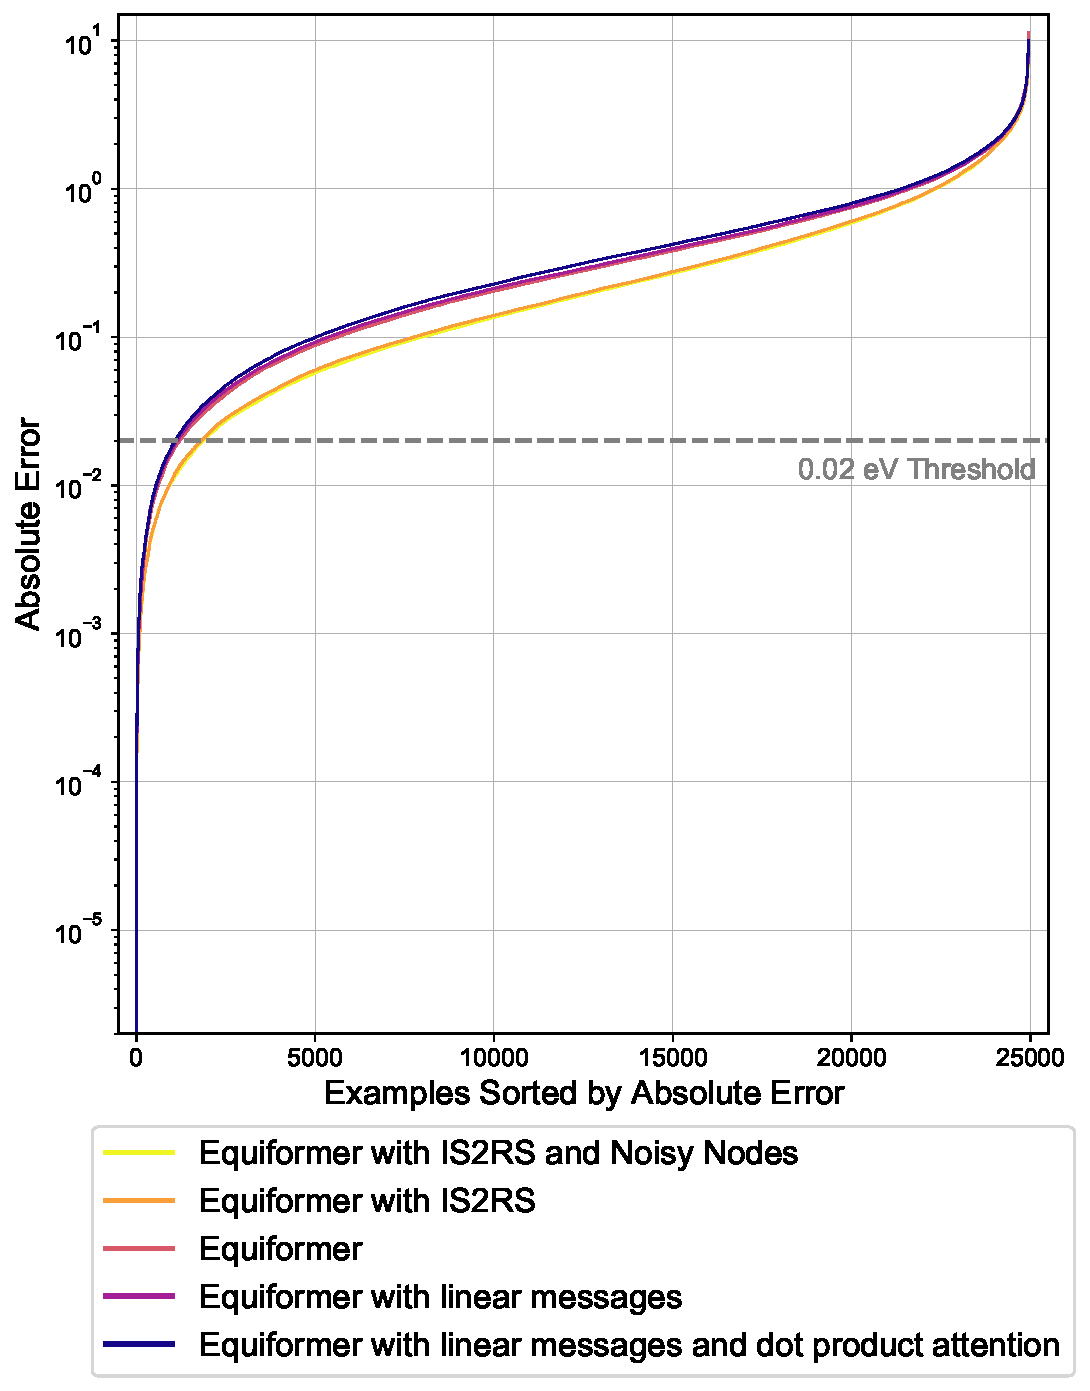
\includegraphics[width=\linewidth]{figure/val_id.pdf}
  \caption{\textbf{ID sub-split.}}
  \vspace{6mm}
  \label{appendix:fig:oc20_val_id}
\end{subfigure}
\begin{subfigure}{.495\textwidth}
  \centering
  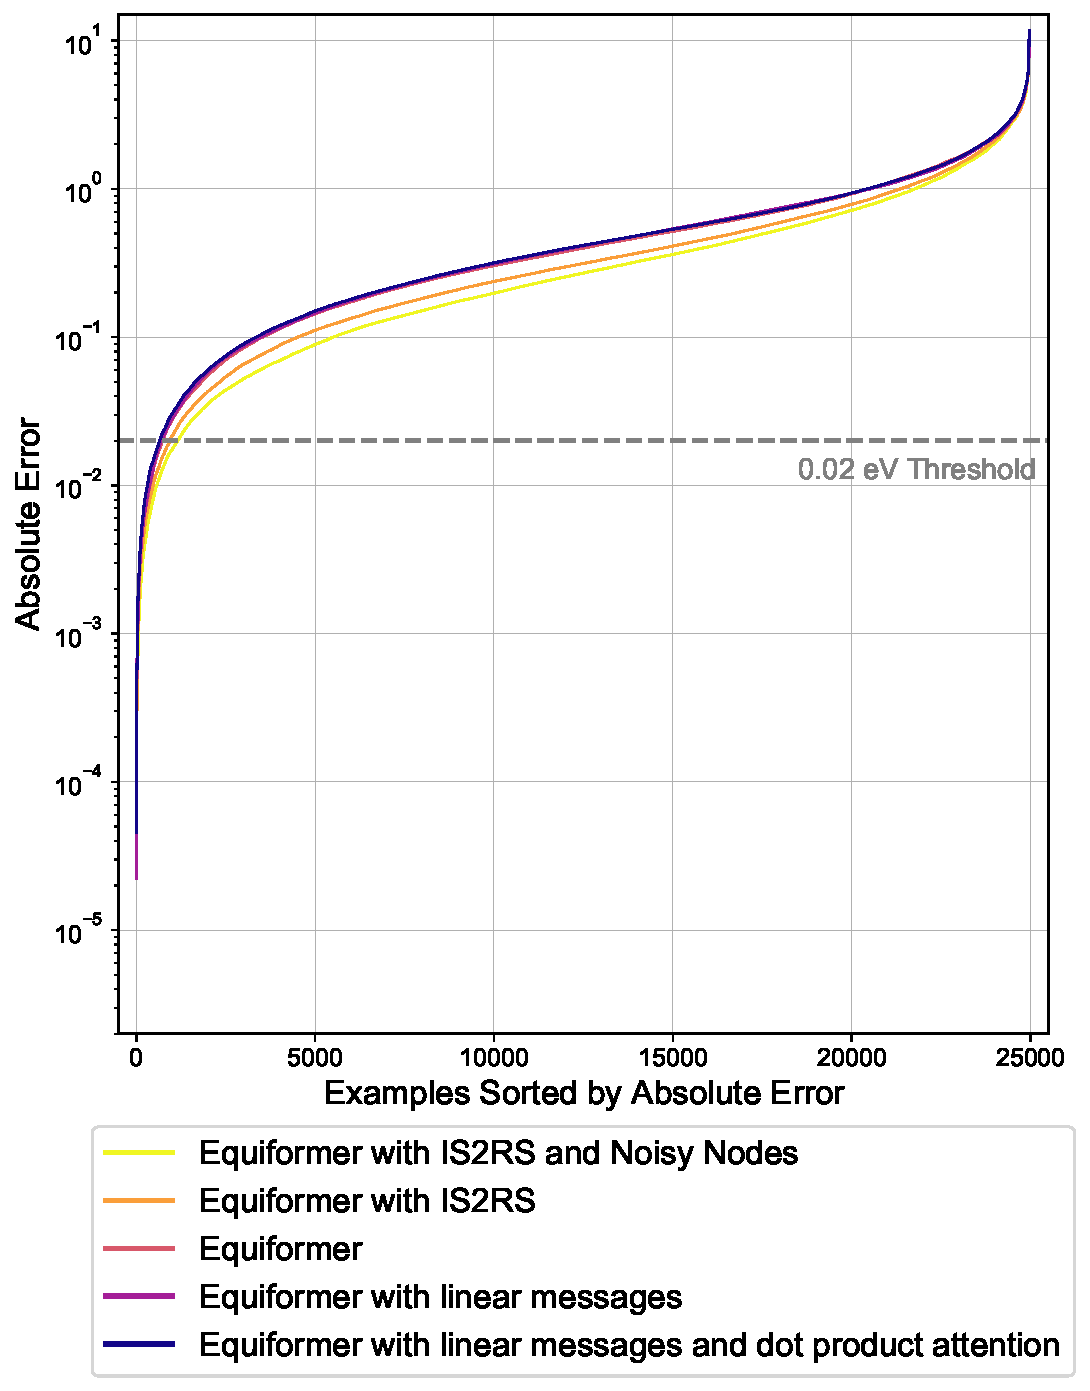
\includegraphics[width=\linewidth]{figure/val_ood_ads.pdf}
  \caption{\textbf{OOD Ads sub-split.}}
  \vspace{6mm}
  \label{appendix:fig:oc20_val_ood_ads}
\end{subfigure}
\begin{subfigure}{.495\textwidth}
  \centering
  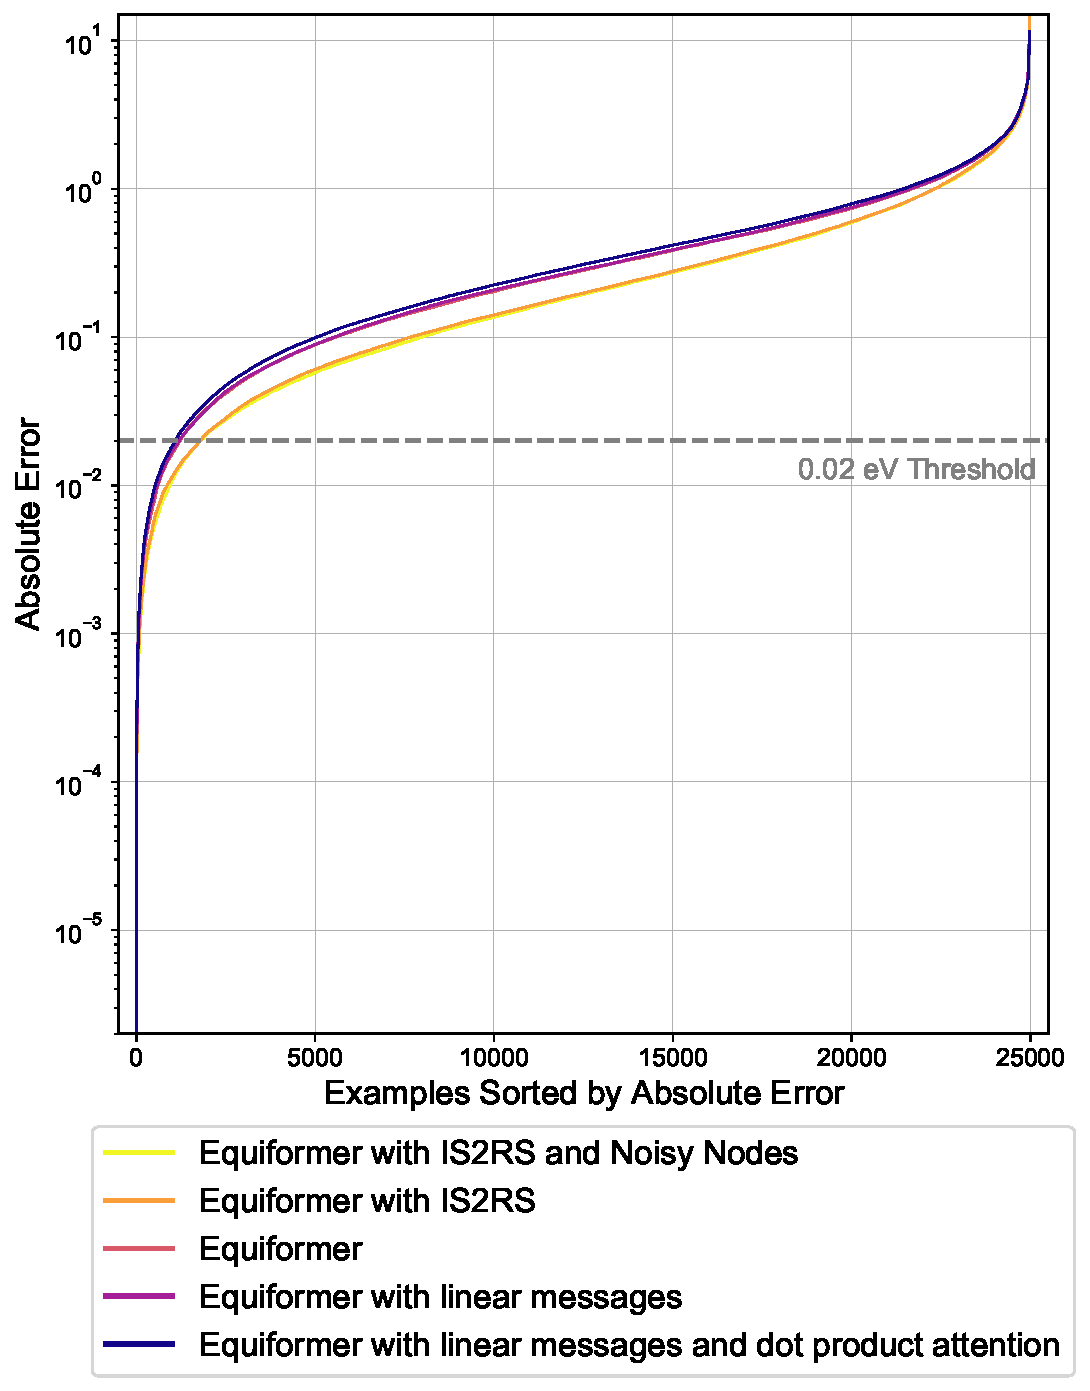
\includegraphics[width=\linewidth]{figure/val_ood_cat.pdf}
  \caption{\textbf{OOD Cat sub-split.}}
  \label{appendix:fig:oc20_val_ood_ads}
\end{subfigure}
\begin{subfigure}{.495\textwidth}
  \centering
  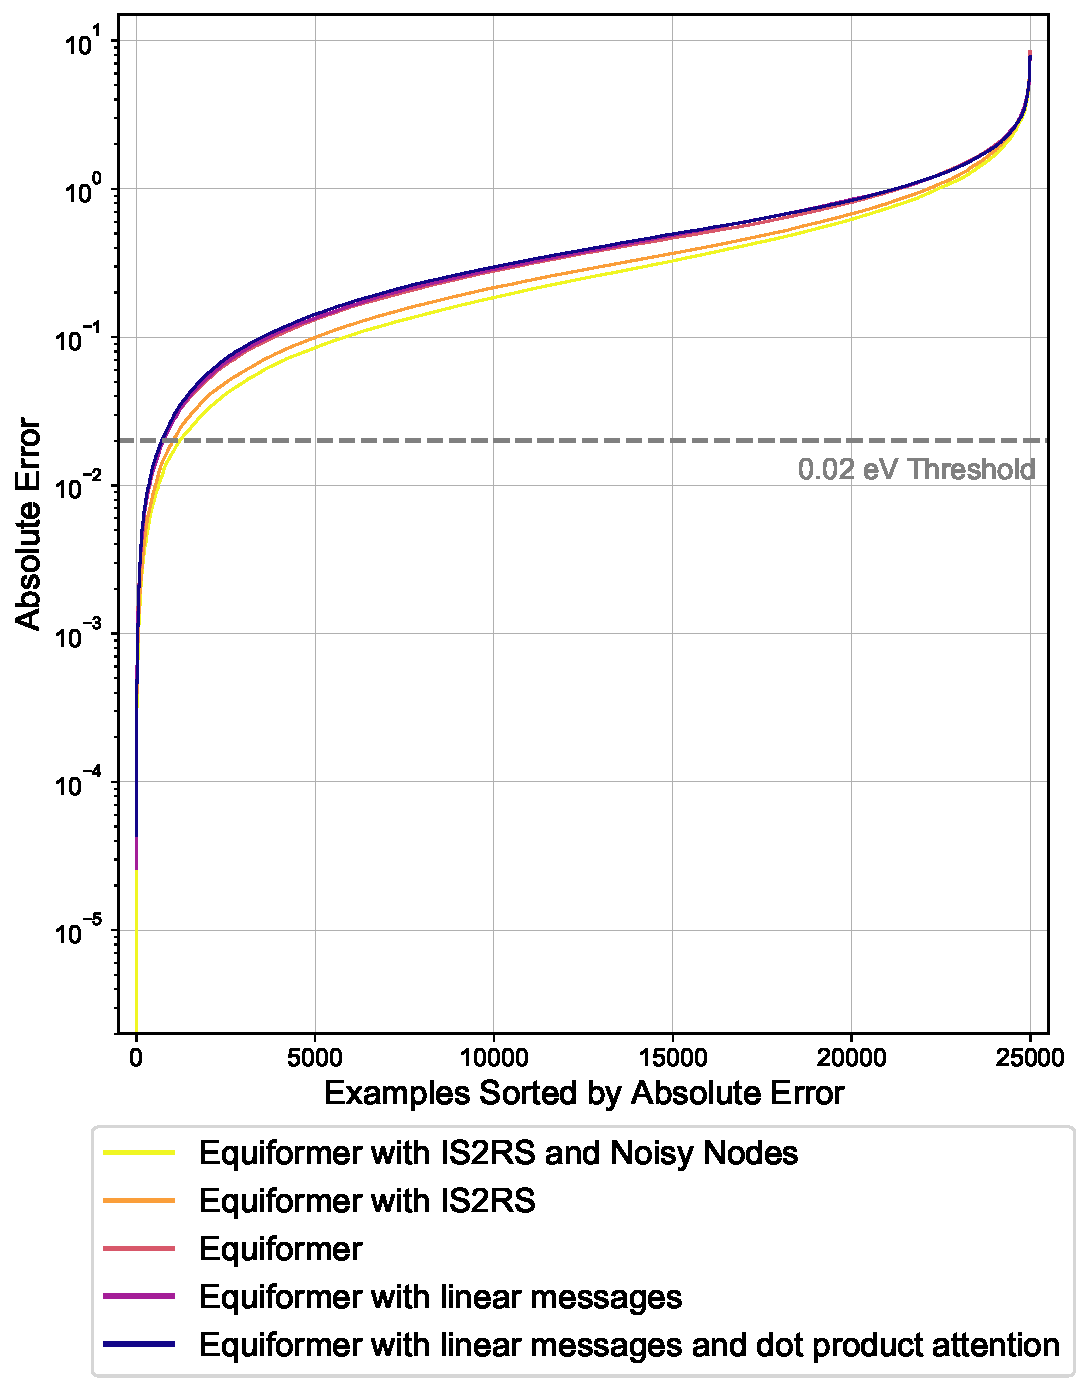
\includegraphics[width=\linewidth]{figure/val_ood_both.pdf}
  \caption{\textbf{OOD Both sub-split.}}
  \label{appendix:fig:oc20_val_ood_ads}
\end{subfigure}
\vspace{4mm}
\caption{\textbf{Error distributions of different Equiformer models on different sub-splits of OC20 IS2RE validation set.} 
%\todo{Examples sorted by error.}
%\todo{Colors of the curves.}
}
\label{appendix:fig:oc20_error_distribution}
\end{figure}

% plot_color_gradients('Perceptually Uniform Sequential',
%                     ['viridis', 'plasma', 'inferno', 'magma', 'cividis'])




\section{Limitations}
\label{appendix:sec:limitations}


We discuss several limitations of the proposed Equiformer and equivariant graph attention below.

First, Equiformer is based on irreducible representations (irreps) and therefore can inherit the limitations common to all equivariant networks based on irreps and the library \texttt{e3nn}~\citep{e3nn}.
For example, using higher degrees $L$ can result in larger features and using tensor products can be compute-intensive. 
Part of the reasons that tensor products can be computationally expensive are that the kernels have not been heavily optimized and customized as other operations in common libraries like PyTorch~\citep{pytorch}. 
But this is the issue related to software, not the design of networks. 
While tensor products of irreps naively do not scale well, if all possible interactions and paths are considered, some paths in tensor products can also be pruned for computational efficiency. 
We leave these potential efficiency gains to future work and in this work focus on general equivariant attention if all possible paths up to $L_{max}$ in tensor products are allowed.

Second,  the improvement of the proposed equivariant graph attention can depend on tasks and datasets. For QM9, MLP attention improves not significantly upon dot product attention as shown in Table~\ref{tab:qm9_ablation}. 
We surmise that this is because QM9 contains less atoms and less diverse atom types and therefore linear attention is enough. For OC20, MLP attention clearly improves upon dot product attention as shown in Table~\ref{tab:oc20_ablation}. Non-linear messages improve upon linear ones for the two datasets.

Third, equivariant graph attention requires more computation than typical graph convolution. 
It includes one softmax operation and thus requires one additional sum aggregation compared to typical message passing. For non-linear message passing, it increases the number of tensor products from one to two and requires more computation. 
We note that if there is a constraint on training budget, using stronger attention (i.e., MLP attention and non-linear messages) would not always be optimal because for some tasks or datasets, the improvement is not that significant and using stronger attention can slow down training. 

%For example, for the task of $C_\nu$ on QM9, using linear (index 2) or non-linear messages (index 1) results in the same performance as shown in Table~\ref{tab:qm9_ablation}.
%However, non-linear messages increase the training time of one epoch from 6.6 minutes to 11 minutes.
%}

Fourth, the proposed attention has complexity proportional to the products of numbers of channels and numbers of edges since the the attention is restricted to local neighborhoods. 
In the context of 3D atomistic graphs, the complexity is the same as that of messages and graph convolutions.
However, in other domains like computer vision, the memory complexity of convolution is proportional to the number of pixels or nodes, not that of edges. 
Therefore, it would require further modifications in order to use the proposed attention in other domains.


